\section{บทที่ 7 การประยุกต์การแปลงลาปลาซในการวิเคราะห์วงจรไฟฟ้า}

\textbf{ชื่อบทภาษาอังกฤษ:} Applications of the Laplace Transform in Electrical Circuit Analysis\\
\textbf{รายวิชา:} คณิตศาสตร์วิศวกรรมไฟฟ้า (Electrical Engineering Mathematics)\\
\textbf{รหัสวิชา:} 5571102

\par\noindent\rule{\textwidth}{0.4pt}\par

\subsection{1. แนวคิดสำคัญของบท}

การแปลงลาปลาซ (Laplace Transform) เป็นเครื่องมือสำคัญที่เชื่อมระหว่าง \textbf{สมการเชิงอนุพันธ์ในโดเมนเวลา} กับ \textbf{สมการพีชคณิตในโดเมนเชิงซ้อน $s$} ทำให้การวิเคราะห์วงจรไฟฟ้าที่มีตัวเก็บประจุและตัวเหนี่ยวนำเป็นระบบมากขึ้น โดยเฉพาะวงจรที่มีการสวิตช์ แหล่งจ่ายแบบขั้นบันได สภาวะเริ่มต้นไม่เป็นศูนย์ และการตอบสนองชั่วครู่

ในวงจรไฟฟ้า ตัวเก็บประจุและตัวเหนี่ยวนำเก็บสะสมพลังงานไว้ในสนามไฟฟ้าและสนามแม่เหล็กตามลำดับ จึงทำให้แรงดันหรือกระแสบางตัวไม่สามารถเปลี่ยนค่าอย่างฉับพลันได้โดยไม่มีแหล่งกระตุ้นเชิงอุดมคติที่เหมาะสม ผลที่ตามมาคือวงจร RC และ RL มีพฤติกรรมอันดับหนึ่ง ส่วนวงจร RLC โดยทั่วไปมีพฤติกรรมอันดับสอง การแปลงลาปลาซช่วยให้เงื่อนไขเริ่มต้นเหล่านี้ถูกนำเข้าไปอยู่ในสมการได้โดยตรง และช่วยให้มองเห็นความสัมพันธ์ระหว่าง \textbf{ค่าคงตัวเวลา (time constant)}, \textbf{ความถี่ธรรมชาติ (natural frequency)}, \textbf{อัตราการหน่วง (damping)}, \textbf{ฟังก์ชันถ่ายโอน (transfer function)} และ \textbf{ตำแหน่งโพล–ซีโร (pole–zero locations)} ได้ชัดเจน

หัวใจของบทนี้ไม่ใช่เพียงการ “แทน $d/dt$ ด้วย $s$” แต่คือการพัฒนากระบวนการวิเคราะห์ที่ถูกต้อง ตั้งแต่การสร้างแบบจำลองวงจร การกำหนดสภาวะก่อนสวิตช์ การใช้กฎของเคอร์ชอฟฟ์ การแปลงสมการไปยังโดเมน $s$ การแก้สมการพีชคณิต การหาลาปลาซผกผัน และการตีความคำตอบกลับมาเป็นพฤติกรรมทางกายภาพของวงจร

\par\noindent\rule{\textwidth}{0.4pt}\par

\subsection{2. ความรู้พื้นฐานก่อนเรียน}

ก่อนเรียนบทนี้ นักศึกษาควรมีความรู้และทักษะต่อไปนี้

\begin{enumerate}
    \item กฎของโอห์ม และกฎแรงดัน–กระแสของเคอร์ชอฟฟ์ (KVL และ KCL)
    \item ความสัมพันธ์แรงดัน–กระแสของตัวต้านทาน ตัวเก็บประจุ และตัวเหนี่ยวนำ
    \item การสร้างสมการเชิงอนุพันธ์อันดับหนึ่งและอันดับสองจากวงจรพื้นฐาน
    \item ความหมายของสภาวะเริ่มต้น เช่น $v_C(0^-)$ และ $i_L(0^-)$
    \item การแปลงลาปลาซของฟังก์ชันพื้นฐาน สมบัติการแปลงอนุพันธ์ และการแปลงลาปลาซผกผัน
    \item การแยกเศษส่วนย่อย (partial fraction expansion)
    \item ฟังก์ชันขั้นบันไดหนึ่งหน่วย $u(t)$ และความสัมพันธ์ $\mathcal{L}\{u(t)\}=1/s$
    \item แนวคิดเบื้องต้นของระบบเชิงเส้นและสมการลักษณะเฉพาะ
\end{enumerate}

\begin{quote}
\textbf{การเชื่อมโยงกับบทที่ 6:} บทที่ 6 เน้นเครื่องมือทางคณิตศาสตร์ของการแปลงลาปลาซ ส่วนบทที่ 7 นำเครื่องมือนั้นมาใช้กับแบบจำลองวงจรจริง โดยต้องตีความทั้งสมการและพฤติกรรมทางไฟฟ้าไปพร้อมกัน
\end{quote}

\par\noindent\rule{\textwidth}{0.4pt}\par

\subsection{3. คำสำคัญประจำบท}

\begin{table}[htbp]
    \centering
    \begin{tabularx}{\textwidth}{L{0.22\textwidth} L{0.22\textwidth} Y}
        \hline
        \textbf{คำศัพท์ภาษาไทย} & \textbf{English term} & \textbf{ความหมายโดยย่อ} \\
        \hline
        โดเมนเวลา & Time Domain & การอธิบายแรงดัน กระแส หรือสัญญาณเป็นฟังก์ชันของเวลา $t$ \\
        โดเมนเอส & $s$-Domain & โดเมนหลังการแปลงลาปลาซ โดยใช้ตัวแปรเชิงซ้อน $s$ \\
        สภาวะเริ่มต้น & Initial Condition & ค่าของพลังงานสะสมในวงจรก่อนหรือขณะเริ่มวิเคราะห์ เช่น $v_C(0^-)$, $i_L(0^-)$ \\
        ค่าคงตัวเวลา & Time Constant & ตัวกำหนดความเร็วของการเปลี่ยนแปลงในระบบอันดับหนึ่ง เช่น $\tau=RC$ หรือ $\tau=L/R$ \\
        การตอบสนองธรรมชาติ & Natural Response & การตอบสนองที่เกิดจากพลังงานเริ่มต้นของวงจรโดยไม่มีแหล่งกระตุ้นใหม่ \\
        การตอบสนองบังคับ & Forced Response & การตอบสนองที่เกิดจากแหล่งกระตุ้นภายนอก \\
        การตอบสนองชั่วครู่ & Transient Response & ส่วนของการตอบสนองที่ลดลงหรือเปลี่ยนแปลงหลังการสวิตช์ก่อนเข้าสู่สภาวะคงตัว \\
        สภาวะคงตัว & Steady-State & พฤติกรรมระยะยาวหลังองค์ประกอบชั่วครู่ลดลงแล้ว \\
        อิมพีแดนซ์ในโดเมน $s$ & $s$-Domain Impedance & ความสัมพันธ์พีชคณิตระหว่างแรงดันและกระแสหลังแปลงลาปลาซภายใต้เงื่อนไขที่กำหนด \\
        ฟังก์ชันถ่ายโอน & Transfer Function & อัตราส่วน $Y(s)/X(s)$ ของระบบเมื่อกำหนดสภาวะเริ่มต้นเป็นศูนย์ \\
        โพล & Pole & รากของพหุนามส่วนตัวส่วนของฟังก์ชันถ่ายโอน \\
        ซีโร & Zero & รากของพหุนามส่วนตัวเศษของฟังก์ชันถ่ายโอน \\
        ความถี่ธรรมชาติ & Natural Frequency & ความถี่เฉพาะของระบบอันดับสอง เช่น $\omega_n=1/\sqrt{LC}$ สำหรับ RLC อนุกรมในรูปมาตรฐาน \\
        อัตราส่วนการหน่วง & Damping Ratio & พารามิเตอร์ไร้มิติ $\zeta$ ที่บอกลักษณะ underdamped, critically damped หรือ overdamped \\
        สมการลักษณะเฉพาะ & Characteristic Equation & สมการที่ได้จากการตั้งพหุนามตัวส่วนเท่ากับศูนย์ ใช้หาโพลของระบบ \\
        \hline
    \end{tabularx}
\end{table}

\par\noindent\rule{\textwidth}{0.4pt}\par

\subsection{4. ผลลัพธ์การเรียนรู้ประจำบท}

\begin{quote}
เมื่อเรียนจบบทนี้ นักศึกษาสามารถ...
\end{quote}

\begin{enumerate}
    \item \textbf{สร้างแบบจำลอง} สมการเชิงอนุพันธ์ของวงจร RC, RL และ RLC จากกฎของเคอร์ชอฟฟ์และความสัมพันธ์ขององค์ประกอบได้
    \item \textbf{แปลงและวิเคราะห์} วงจรไฟฟ้าจากโดเมนเวลาไปสู่โดเมน $s$ โดยคำนึงถึงสภาวะเริ่มต้นได้อย่างถูกต้อง
    \item \textbf{คำนวณ} แรงดันและกระแสของวงจร RC, RL และ RLC เมื่อได้รับอินพุตแบบขั้นบันไดหรือมีพลังงานเริ่มต้นได้
    \item \textbf{จำแนกและอธิบาย} การตอบสนองธรรมชาติ การตอบสนองบังคับ การตอบสนองชั่วครู่ และการตอบสนองสภาวะคงตัวได้
    \item \textbf{หาและตีความ} ฟังก์ชันถ่ายโอนของวงจรไฟฟ้าพื้นฐาน รวมถึงโพล ซีโร ค่าคงตัวเวลา และพารามิเตอร์อันดับสองได้
    \item \textbf{ประเมิน} ลักษณะเสถียรภาพและรูปทรงการตอบสนองของวงจรจากตำแหน่งโพลในระนาบ $s$ ได้ในระดับเบื้องต้น
\end{enumerate}

\subsubsection{4.1 ตารางความสอดคล้องแบบ OBE}

\begin{table}[htbp]
    \centering
    \small
    \setlength{\tabcolsep}{4pt}
    \begin{tabularx}{\textwidth}{L{0.18\textwidth} L{0.12\textwidth} L{0.21\textwidth} L{0.17\textwidth} Y}
        \hline
        \textbf{ผลลัพธ์การเรียนรู้ประจำบท} & \textbf{เนื้อหาที่เกี่ยวข้อง} & \textbf{กิจกรรมการเรียนรู้} & \textbf{วิธีประเมิน} & \textbf{หลักฐานการเรียนรู้} \\
        \hline
        CLO1 สร้างแบบจำลอง RC/RL/RLC & 7.1–7.2 & วิเคราะห์วงจรจากแผนภาพและเขียน KVL/KCL & แบบฝึกหัดสร้างสมการ & สมการเชิงอนุพันธ์พร้อมกำหนดตัวแปรและหน่วย \\
        CLO2 แปลงวงจรสู่โดเมน $s$ & 7.3–7.4 & จับคู่สมการเวลาและสมการใน $s$ & แบบฝึกหัดระหว่างเรียน & วงจรสมมูลและสมการพีชคณิตใน $s$ \\
        CLO3 คำนวณการตอบสนอง RC/RL/RLC & 7.5–7.7 & ตัวอย่างคำนวณแบบเป็นขั้นตอน & แบบฝึกหัดคำนวณ & คำตอบ $v(t)$ หรือ $i(t)$ พร้อมตรวจสอบค่าเริ่มต้น/ปลายทาง \\
        CLO4 จำแนกองค์ประกอบการตอบสนอง & 7.8 & วิเคราะห์กราฟและแยก natural/forced & คำถามอธิบายและอภิปราย & แผนภาพหรือคำอธิบายเชิงเหตุผล \\
        CLO5 หา transfer function และ pole–zero & 7.9–7.10 & หา $G(s)$ จากวงจรและระบุราก & แบบฝึกหัดวิเคราะห์ & ฟังก์ชันถ่ายโอน แผนภาพ pole–zero และการตีความ \\
        CLO6 ประเมินเสถียรภาพเบื้องต้น & 7.10–9 & กรณีศึกษาเปรียบเทียบตำแหน่งโพล & แบบฝึกหัดระดับประยุกต์ & ข้อสรุปเสถียรภาพและเหตุผลจากตำแหน่งโพล \\
        \hline
    \end{tabularx}
\end{table}

\par\noindent\rule{\textwidth}{0.4pt}\par

\subsection{5. แผนผังเนื้อหาของบท}

ลำดับการเรียนรู้ของบทนี้สามารถสรุปได้ดังนี้

\textbf{วงจรจริงและการสวิตช์}\\
$\downarrow$\\
\textbf{กำหนดตัวแปร ทิศทาง และสภาวะเริ่มต้น}\\
$\downarrow$\\
\textbf{ใช้ KVL/KCL + ความสัมพันธ์ $R,L,C$}\\
$\downarrow$\\
\textbf{ได้สมการเชิงอนุพันธ์ในโดเมนเวลา}\\
$\downarrow$\\
\textbf{ใช้การแปลงลาปลาซ}\\
$\downarrow$\\
\textbf{ได้สมการพีชคณิตและอิมพีแดนซ์ในโดเมน $s$}\\
$\downarrow$\\
\textbf{แก้หา $V(s)$ หรือ $I(s)$}\\
$\downarrow$\\
\textbf{แยกเศษส่วนย่อยและหาลาปลาซผกผัน}\\
$\downarrow$\\
\textbf{ได้ $v(t)$ หรือ $i(t)$ และตรวจสอบค่าเริ่มต้น/สภาวะคงตัว}\\
$\downarrow$\\
\textbf{สร้างฟังก์ชันถ่ายโอนและวิเคราะห์ pole–zero}\\
$\downarrow$\\
\textbf{ตีความ transient response และเสถียรภาพ}

% [รูปที่ 1: แผนภาพแนวคิดการวิเคราะห์วงจรด้วยการแปลงลาปลาซ]
% ประเภทภาพ: Flowchart / Infographic
% ตำแหน่งที่แนะนำ: หลังหัวข้อ 5 แผนผังเนื้อหาของบท
% วัตถุประสงค์การเรียนรู้: ช่วยให้ผู้เรียนเห็นความสัมพันธ์ระหว่างวงจรจริง สมการเชิงอนุพันธ์ โดเมน $s$ และการตีความคำตอบ
% คำอธิบายภาพ: แสดงลำดับจาก circuit diagram → KVL/KCL → differential equation → Laplace transform → algebraic $s$-domain circuit → solve $V(s),I(s)$ → inverse Laplace → time response → transfer function/poles/zeros พร้อมลูกศรทิศทางเดียวและวงรอบตรวจสอบ initial/final values
% องค์ประกอบที่ต้องมี: ตัวต้านทาน ตัวเก็บประจุ ตัวเหนี่ยวนำ สวิตช์ กล่องสมการ $d/dt$ กล่อง $s$-domain กล่อง inverse Laplace ระนาบ $s$ และกราฟ response
% ข้อความหรือป้ายกำกับ: “Time Domain”, “Initial Conditions”, “Laplace Transform”, “$s$-Domain”, “Inverse Laplace”, “Transient Response”, “Transfer Function”, “Poles/Zeros”
% ภาษาของป้ายกำกับ: ไทยและอังกฤษ
% สัดส่วนภาพ: 16:9
% Image Generation Prompt: Clean engineering textbook flowchart showing the complete workflow for Laplace-transform circuit analysis: physical RC/RL/RLC circuit with switch, define initial conditions, apply KVL/KCL, form differential equation in time domain, apply Laplace transform, obtain algebraic s-domain circuit, solve V(s) or I(s), perform inverse Laplace transform, obtain time response, then derive transfer function and interpret poles and zeros. Include a small verification loop for initial and final values. White background, precise electrical symbols, bilingual Thai-English labels, vector textbook style, 16:9.
% Graph Generation Prompt: Not applicable.
% Alt Text: ผังงานแสดงขั้นตอนการวิเคราะห์วงจร RC/RL/RLC ตั้งแต่สมการเวลา ผ่านการแปลงลาปลาซ ไปจนถึงการตอบสนองเวลาและการวิเคราะห์โพล–ซีโร

\begin{figure}[htbp]
    \centering
    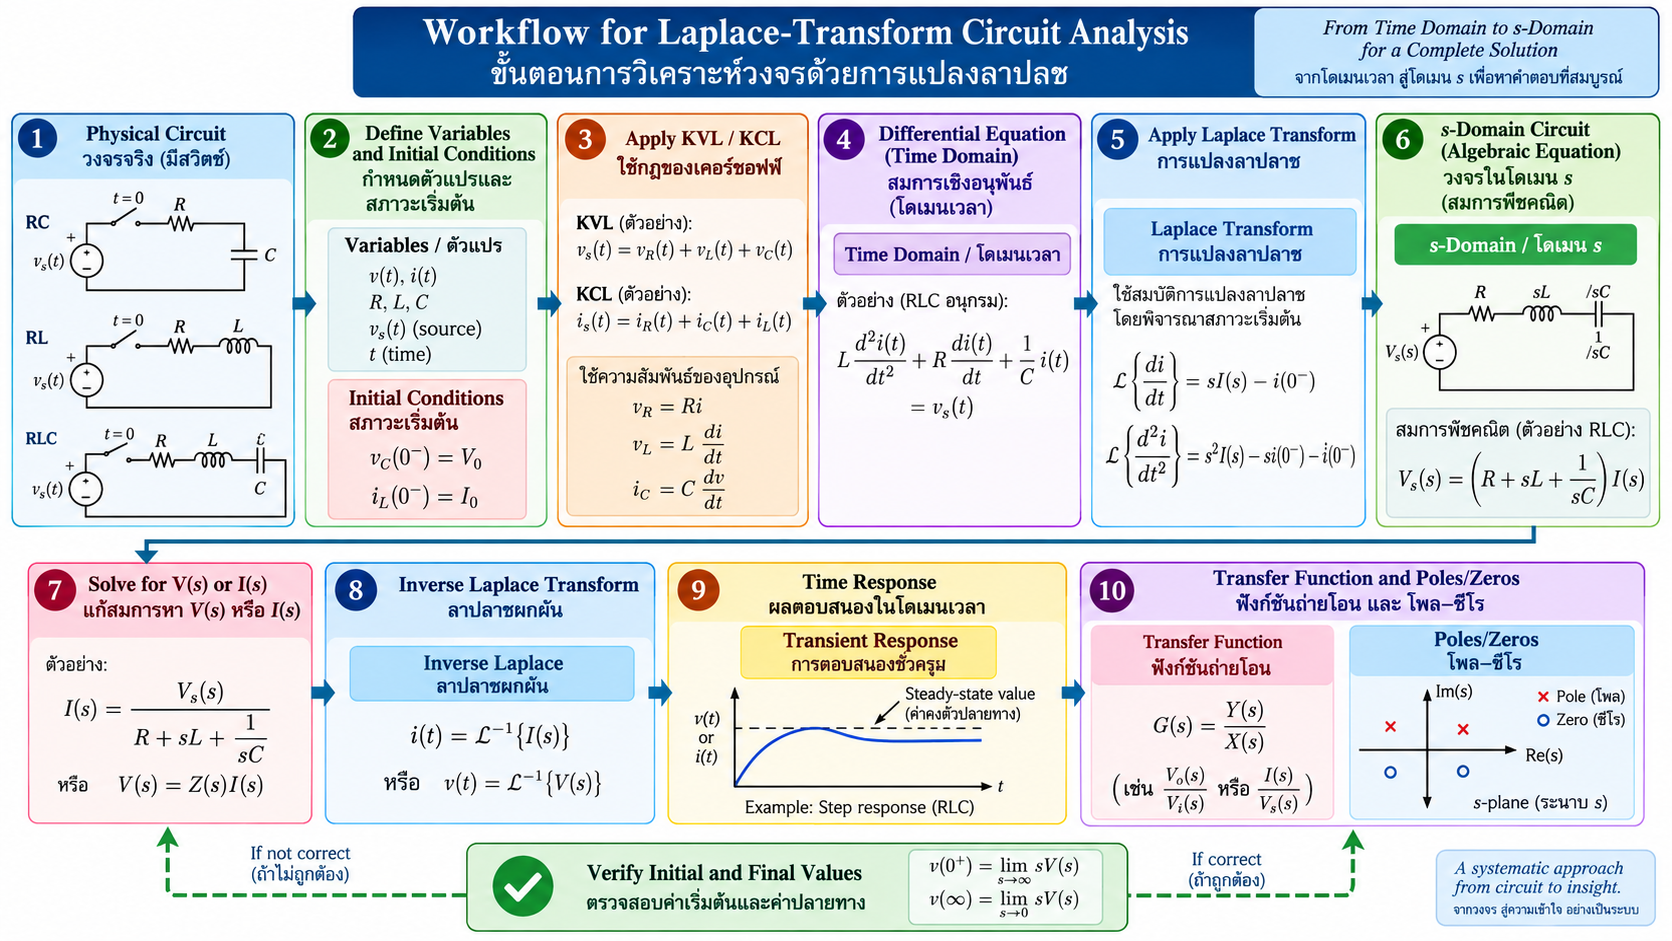
\includegraphics[width=0.8\textwidth]{images/chapter7/figure-01.png}
    \caption{แผนภาพแนวคิดการวิเคราะห์วงจรด้วยการแปลงลาปลาซ}
\end{figure}

\par\noindent\rule{\textwidth}{0.4pt}\par

\subsection{6. บทนำ}

ในวิชาวงจรไฟฟ้าพื้นฐาน นักศึกษามักเริ่มต้นจากวงจรที่อยู่ในสภาวะคงตัว เช่น วงจรตัวต้านทานกระแสตรง หรือวงจรกระแสสลับแบบไซน์ที่ใช้เฟสเซอร์ได้โดยตรง แต่ระบบจริงจำนวนมากไม่ได้ทำงานอยู่ในสภาวะคงตัวตลอดเวลา เมื่อมีการเปิด–ปิดสวิตช์ การต่อแหล่งจ่ายใหม่ การเปลี่ยนโหลด หรือการเปลี่ยนสัญญาณอินพุต พลังงานที่เก็บอยู่ในตัวเก็บประจุและตัวเหนี่ยวนำทำให้แรงดันและกระแสต้องเปลี่ยนผ่านช่วงหนึ่งก่อนเข้าสู่สภาวะใหม่ ช่วงนี้เรียกว่า \textbf{การตอบสนองชั่วครู่ (transient response)}

หากวิเคราะห์ในโดเมนเวลาโดยตรง วงจร RC และ RL นำไปสู่สมการเชิงอนุพันธ์อันดับหนึ่ง ส่วน RLC นำไปสู่สมการอันดับสอง วิธีแก้สมการโดยตรงสามารถทำได้ แต่เมื่อวงจรซับซ้อนขึ้น มีหลายแหล่งจ่าย หรือมีสภาวะเริ่มต้นไม่เป็นศูนย์ การจัดการสมการจะยุ่งยากขึ้น การแปลงลาปลาซจึงมีคุณค่าเพราะเปลี่ยนปัญหาจาก “การแก้สมการเชิงอนุพันธ์” เป็น “การแก้สมการพีชคณิตในตัวแปร $s$” และยังรวมผลของสภาวะเริ่มต้นเข้าไปในสมการได้

สำหรับวงจรอันดับหนึ่ง MIT OpenCourseWare อธิบายว่า transient คือพฤติกรรมระหว่างการเปลี่ยนจากสภาวะคงตัวหนึ่งไปสู่อีกสภาวะหนึ่ง และแสดงให้เห็นว่าผลคูณ $RC$ และอัตราส่วน $L/R$ มีหน่วยเป็นเวลาและทำหน้าที่เป็นค่าคงตัวเวลาของวงจร ขณะที่วงจร RLC มีพฤติกรรมอันดับสองซึ่งขึ้นกับความสัมพันธ์ระหว่างอัตราการหน่วงกับความถี่ธรรมชาติ ทั้งสามกรณีนี้เป็นแกนสำคัญของบทเรียนนี้

\par\noindent\rule{\textwidth}{0.4pt}\par

\subsection{7. เนื้อหาหลัก}

\subsubsection{7.1 แบบจำลองทางคณิตศาสตร์ของวงจรไฟฟ้า}

การวิเคราะห์ด้วยลาปลาซเริ่มต้นจาก \textbf{แบบจำลองที่ถูกต้องในโดเมนเวลา} หากสมการตั้งต้นผิด การแปลงลาปลาซจะเพียงเปลี่ยนรูปของข้อผิดพลาดเท่านั้น ดังนั้นนักศึกษาควรเริ่มจากการกำหนดตัวแปรและทิศทางให้ชัดเจน

\paragraph{7.1.1 ความสัมพันธ์ขององค์ประกอบพื้นฐาน}

สำหรับตัวต้านทาน $R$ ภายใต้ passive sign convention

\[
v_R(t)=R i_R(t)
\]

\begin{itemize}
    \item $v_R(t)$ คือแรงดันคร่อมตัวต้านทาน หน่วยโวลต์ (V)
    \item $i_R(t)$ คือกระแสผ่านตัวต้านทาน หน่วยแอมแปร์ (A)
    \item $R$ คือความต้านทาน หน่วยโอห์ม ($\Omega$)
\end{itemize}

สมการนี้เป็นความสัมพันธ์พีชคณิต ไม่มีการเก็บสะสมพลังงานในตัวต้านทานอุดมคติ

สำหรับตัวเก็บประจุ $C$

\[
i_C(t)=C\frac{dv_C(t)}{dt}
\]

หรือ

\[
v_C(t)=v_C(t_0)+\frac{1}{C}\int_{t_0}^{t}i_C(\lambda)\,d\lambda
\]

\begin{itemize}
    \item $C$ มีหน่วยฟารัด (F)
    \item แรงดัน $v_C$ สัมพันธ์กับพลังงานสะสม $W_C=\tfrac{1}{2}Cv_C^2$
\end{itemize}

สำหรับตัวเหนี่ยวนำ $L$

\[
v_L(t)=L\frac{di_L(t)}{dt}
\]

หรือ

\[
i_L(t)=i_L(t_0)+\frac{1}{L}\int_{t_0}^{t}v_L(\lambda)\,d\lambda
\]

\begin{itemize}
    \item $L$ มีหน่วยเฮนรี (H)
    \item กระแส $i_L$ สัมพันธ์กับพลังงานสะสม $W_L=\tfrac{1}{2}Li_L^2$
\end{itemize}

\paragraph{7.1.2 ความต่อเนื่องของตัวแปรพลังงาน}

ในวงจรอุดมคติทั่วไปที่ไม่มีอิมพัลส์อนันต์มากระทำ

\[
v_C(0^+)=v_C(0^-)
\]

และ

\[
i_L(0^+)=i_L(0^-)
\]

ข้อความนี้มีความหมายว่า \textbf{แรงดันตัวเก็บประจุไม่กระโดดโดยฉับพลัน} และ \textbf{กระแสตัวเหนี่ยวนำไม่กระโดดโดยฉับพลัน} เนื่องจากการเปลี่ยนค่าอย่างฉับพลันจะต้องการอนุพันธ์เป็นอิมพัลส์และเกี่ยวข้องกับแรงดันหรือกระแสอุดมคติที่สูงมาก

อย่างไรก็ตาม กระแสของตัวเก็บประจุสามารถเปลี่ยนทันทีได้ และแรงดันของตัวเหนี่ยวนำสามารถเปลี่ยนทันทีได้ตามเครือข่ายที่ต่ออยู่ จึงต้องระวังไม่สลับคู่ตัวแปรที่ต่อเนื่อง

\paragraph{7.1.3 ขั้นตอนตั้งแบบจำลอง}

\begin{enumerate}
    \item วาดวงจรก่อนสวิตช์ $t<0$ และหลังสวิตช์ $t>0$
    \item หา $v_C(0^-)$ และ $i_L(0^-)$ จากสภาวะก่อนสวิตช์
    \item ใช้ความต่อเนื่องเพื่อหา $v_C(0^+)$ และ $i_L(0^+)$
    \item กำหนดทิศทางกระแสและขั้วแรงดัน
    \item ใช้ KVL หรือ KCL กับวงจรหลังสวิตช์
    \item แทนความสัมพันธ์ของ $R,L,C$
    \item จัดรูปเป็นสมการเชิงอนุพันธ์มาตรฐาน
    \item ตรวจสอบหน่วยและอันดับของสมการ
\end{enumerate}

% [รูปที่ 2: ตัวแปรที่ต่อเนื่องของตัวเก็บประจุและตัวเหนี่ยวนำขณะสวิตช์]
% ประเภทภาพ: Technical Illustration
% ตำแหน่งที่แนะนำ: หัวข้อ 7.1.2
% วัตถุประสงค์การเรียนรู้: ป้องกันความเข้าใจผิดเรื่องค่า $0^-$ และ $0^+$ ของ $v_C$ และ $i_L$
% คำอธิบายภาพ: แบ่งภาพเป็นสองแผง แผงซ้ายเป็น capacitor ก่อนและหลังสวิตช์ แสดง $v_C(0^-)=v_C(0^+)$ และกระแสที่อาจเปลี่ยนได้ แผงขวาเป็น inductor แสดง $i_L(0^-)=i_L(0^+)$ และแรงดันที่อาจเปลี่ยนได้
% องค์ประกอบที่ต้องมี: สวิตช์ สัญลักษณ์ C และ L เส้นเวลา $0^-,0^+$ ลูกศรแรงดัน/กระแส และป้าย “continuous variable”
% ข้อความหรือป้ายกำกับ: “Capacitor voltage is continuous”, “Inductor current is continuous”, “ก่อนสวิตช์ $0^-$”, “หลังสวิตช์ $0^+$”
% ภาษาของป้ายกำกับ: ไทยและอังกฤษ
% สัดส่วนภาพ: 16:9
% Image Generation Prompt: Two-panel engineering textbook illustration about switching initial conditions. Left panel: capacitor circuit before and after t=0, showing v_C(0-)=v_C(0+) as the continuous state variable while capacitor current may change. Right panel: inductor circuit before and after t=0, showing i_L(0-)=i_L(0+) while inductor voltage may change. Include a small time-axis around 0-, 0+, correct electrical symbols and polarity arrows. Clean white background, bilingual Thai-English labels, precise vector style, 16:9.
% Graph Generation Prompt: Not applicable.
% Alt Text: ภาพเปรียบเทียบเงื่อนไขต่อเนื่องของแรงดันตัวเก็บประจุและกระแสตัวเหนี่ยวนำในช่วงก่อนและหลังสวิตช์

\begin{figure}[htbp]
    \centering
    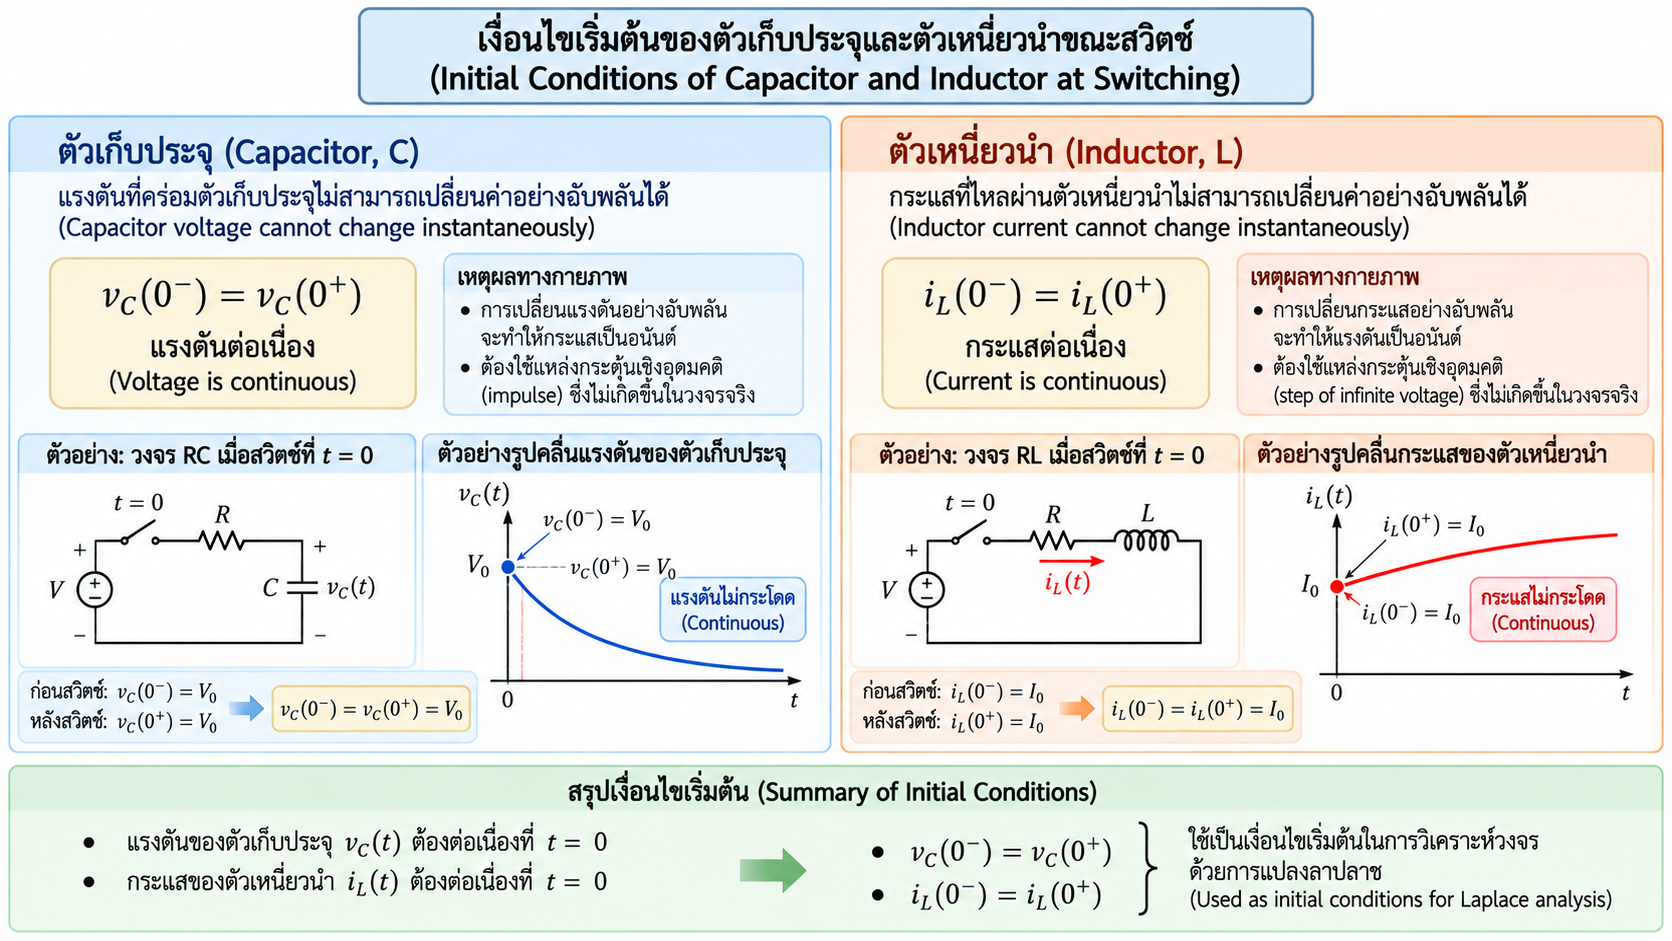
\includegraphics[width=0.8\textwidth]{images/chapter7/figure-02.png}
    \caption{ตัวแปรที่ต่อเนื่องของตัวเก็บประจุและตัวเหนี่ยวนำขณะสวิตช์}
\end{figure}

\par\noindent\rule{\textwidth}{0.4pt}\par

\subsubsection{7.2 สมการเชิงอนุพันธ์ของวงจร RC, RL และ RLC}

\paragraph{7.2.1 วงจร RC อนุกรม}

พิจารณาแหล่งแรงดัน $v_s(t)$ ต่ออนุกรมกับ $R$ และ $C$ และกำหนดเอาต์พุตเป็น $v_C(t)$ จาก KVL

\[
v_s(t)=v_R(t)+v_C(t)
\]

เนื่องจาก

\[
v_R(t)=Ri(t), \qquad i(t)=C\frac{dv_C(t)}{dt}
\]

จึงได้

\[
RC\frac{dv_C(t)}{dt}+v_C(t)=v_s(t)
\]

สมการนี้เป็นสมการเชิงอนุพันธ์อันดับหนึ่ง หากพิจารณาวงจรไม่มีแหล่งจ่ายหลังสวิตช์ $v_s=0$ จะได้สมการธรรมชาติ

\[
RC\frac{dv_C(t)}{dt}+v_C(t)=0
\]

ค่าคงตัวเวลา

\[
\tau_{RC}=RC
\]

หน่วยของ $RC$ คือวินาที เนื่องจาก $\Omega\cdot\mathrm{F}=\mathrm{s}$

\textbf{ความหมายทางกายภาพ:} หลังเวลาประมาณหนึ่งค่าคงตัวเวลา การตอบสนองเอ็กซ์โพเนนเชียลจะเคลื่อนจากค่าเริ่มต้นไปยังค่าปลายทางประมาณ $63.2\%$ ของระยะทั้งหมด หรือเหลือส่วนต่างจากค่าปลายทางประมาณ $36.8\%$

\paragraph{7.2.2 วงจร RL อนุกรม}

จาก KVL

\[
v_s(t)=Ri(t)+L\frac{di(t)}{dt}
\]

หรือ

\[
L\frac{di(t)}{dt}+Ri(t)=v_s(t)
\]

เมื่อไม่มีแหล่งจ่ายหลังสวิตช์

\[
L\frac{di(t)}{dt}+Ri(t)=0
\]

ค่าคงตัวเวลา

\[
\tau_{RL}=\frac{L}{R}
\]

โดย $L/R$ มีหน่วยวินาที

\paragraph{7.2.3 วงจร RLC อนุกรม}

พิจารณาวงจร $R$–$L$–$C$ อนุกรม และเลือกแรงดันตัวเก็บประจุ $v_C(t)$ เป็นเอาต์พุต กระแสในวงจรคือ

\[
i(t)=C\frac{dv_C(t)}{dt}
\]

แรงดันตัวเหนี่ยวนำคือ

\[
v_L(t)=L\frac{di(t)}{dt}=LC\frac{d^2v_C(t)}{dt^2}
\]

และแรงดันตัวต้านทานคือ

\[
v_R(t)=RC\frac{dv_C(t)}{dt}
\]

จาก KVL

\[
v_L(t)+v_R(t)+v_C(t)=v_s(t)
\]

จึงได้

\[
LC\frac{d^2v_C(t)}{dt^2}+RC\frac{dv_C(t)}{dt}+v_C(t)=v_s(t)
\]

หารด้วย $LC$

\[
\frac{d^2v_C(t)}{dt^2}+\frac{R}{L}\frac{dv_C(t)}{dt}+\frac{1}{LC}v_C(t)=\frac{1}{LC}v_s(t)
\]

เมื่อเปรียบเทียบกับรูปมาตรฐานอันดับสอง

\[
\frac{d^2y}{dt^2}+2\zeta\omega_n\frac{dy}{dt}+\omega_n^2y=\omega_n^2x(t)
\]

จะได้

\[
\omega_n=\frac{1}{\sqrt{LC}}
\]

\[
\alpha=\frac{R}{2L}
\]

และ

\[
\zeta=\frac{\alpha}{\omega_n}=\frac{R}{2}\sqrt{\frac{C}{L}}
\]

โดย

\begin{itemize}
    \item $\omega_n$ คือความถี่ธรรมชาติ หน่วย rad/s
    \item $\alpha$ คืออัตราการลดทอนของซองเอ็กซ์โพเนนเชียล หน่วย s$^{-1}$
    \item $\zeta$ คืออัตราส่วนการหน่วง ไม่มีหน่วย
\end{itemize}

สำหรับวงจร RLC อนุกรม

\begin{itemize}
    \item $\zeta<1$ หรือ $\alpha<\omega_n$ : \textbf{Underdamped} มีการสั่นที่ค่อย ๆ ลดลง
    \item $\zeta=1$ หรือ $\alpha=\omega_n$ : \textbf{Critically damped} กลับสู่สมดุลเร็วโดยไม่สั่น
    \item $\zeta>1$ หรือ $\alpha>\omega_n$ : \textbf{Overdamped} ไม่สั่น แต่โดยทั่วไปช้ากว่า critical damping
\end{itemize}

ค่าความต้านทานวิกฤตคือ

\[
R_{\text{crit}}=2\sqrt{\frac{L}{C}}
\]

สมการนี้ใช้กับวงจร \textbf{RLC อนุกรมตามแบบจำลองที่กำหนด} เท่านั้น ไม่ควรนำไปใช้กับวงจร RLC แบบขนานโดยตรง เพราะพารามิเตอร์การหน่วงมีรูปต่างกัน

\par\noindent\rule{\textwidth}{0.4pt}\par

\subsubsection{7.3 การแปลงวงจรจากโดเมนเวลาไปสู่โดเมน \texorpdfstring{$s$}{s}}

\paragraph{7.3.1 สมบัติการแปลงอนุพันธ์}

หาก $F(s)=\mathcal{L}\{f(t)\}$ แล้ว

\[
\mathcal{L}\left\{\frac{df(t)}{dt}\right\}=sF(s)-f(0^-)
\]

และ

\[
\mathcal{L}\left\{\frac{d^2f(t)}{dt^2}\right\}=s^2F(s)-sf(0^-)-f'(0^-)
\]

สองสมการนี้คือเหตุผลสำคัญที่การแปลงลาปลาซเหมาะกับปัญหาสวิตช์ เพราะ \textbf{เงื่อนไขเริ่มต้นเข้าสู่สมการโดยตรง}

\paragraph{7.3.2 ตัวต้านทานในโดเมน $s$}

จาก

\[
v_R(t)=Ri_R(t)
\]

แปลงลาปลาซได้

\[
V_R(s)=RI_R(s)
\]

ดังนั้น

\[
Z_R(s)=R
\]

\paragraph{7.3.3 ตัวเหนี่ยวนำในโดเมน $s$}

จาก

\[
v_L(t)=L\frac{di_L(t)}{dt}
\]

แปลงลาปลาซได้

\[
V_L(s)=L\left[sI_L(s)-i_L(0^-)\right]
\]

หรือ

\[
V_L(s)=sLI_L(s)-Li_L(0^-)
\]

เมื่อ $i_L(0^-)=0$

\[
Z_L(s)=sL
\]

หาก $i_L(0^-)\neq0$ เทอม $Li_L(0^-)$ ต้องคงอยู่ในสมการ หรือสามารถแทนด้วยแหล่งกำเนิดสมมูลในวงจร $s$-domain โดยต้องรักษาขั้วตามสมการที่เลือก

\paragraph{7.3.4 ตัวเก็บประจุในโดเมน $s$}

จาก

\[
i_C(t)=C\frac{dv_C(t)}{dt}
\]

แปลงลาปลาซได้

\[
I_C(s)=C\left[sV_C(s)-v_C(0^-)\right]
\]

หรือ

\[
I_C(s)=sCV_C(s)-Cv_C(0^-)
\]

แก้หาแรงดัน

\[
V_C(s)=\frac{1}{sC}I_C(s)+\frac{v_C(0^-)}{s}
\]

เมื่อ $v_C(0^-)=0$

\[
Z_C(s)=\frac{1}{sC}
\]

\textbf{ข้อควรระวัง:} การเขียนเพียง $Z_L=sL$ และ $Z_C=1/(sC)$ โดยไม่พิจารณาสภาวะเริ่มต้น ถูกต้องเฉพาะกรณีที่พลังงานเริ่มต้นเป็นศูนย์ หรือเมื่อผลของสภาวะเริ่มต้นถูกแทนด้วยแหล่งสมมูลไว้อย่างถูกต้องแล้ว

% [รูปที่ 3: แบบจำลององค์ประกอบ R, L และ C ในโดเมนเวลาและโดเมน $s$]
% ประเภทภาพ: Technical Illustration / Circuit Diagram
% ตำแหน่งที่แนะนำ: หัวข้อ 7.3.2–7.3.4
% วัตถุประสงค์การเรียนรู้: ช่วยให้ผู้เรียนเชื่อมความสัมพันธ์เชิงอนุพันธ์กับอิมพีแดนซ์และเทอมสภาวะเริ่มต้น
% คำอธิบายภาพ: ตารางภาพ 3 แถวสำหรับ R, L, C แสดง time-domain equation ทางซ้าย และ s-domain equation ทางขวา โดยแยกกรณี zero initial conditions ออกจาก nonzero initial conditions
% องค์ประกอบที่ต้องมี: สัญลักษณ์ R/L/C, $V(s)$, $I(s)$, $R$, $sL$, $1/(sC)$, เทอม $Li_L(0^-)$ และ $v_C(0^-)/s$
% ข้อความหรือป้ายกำกับ: “Zero Initial Condition”, “Nonzero Initial Condition”, “Time Domain”, “s-Domain”
% ภาษาของป้ายกำกับ: ไทยและอังกฤษ
% สัดส่วนภาพ: 16:9
% Image Generation Prompt: Engineering textbook comparison diagram of resistor, inductor and capacitor models in the time domain versus the Laplace s-domain. Show R: V=RI and Z=R; L: V=sLI-L i(0-) and zero-initial impedance sL; C: I=sCV-Cv(0-) and equivalent V=I/(sC)+v(0-)/s with zero-initial impedance 1/(sC). Clearly separate zero initial conditions from nonzero initial conditions. Use correct circuit symbols, polarity and current arrows, clean white background, bilingual Thai-English labels, vector style, 16:9.
% Graph Generation Prompt: Not applicable.
% Alt Text: แผนภาพเปรียบเทียบสมการของ R, L และ C ก่อนและหลังการแปลงลาปลาซ พร้อมเทอมเงื่อนไขเริ่มต้น

\begin{figure}[htbp]
    \centering
    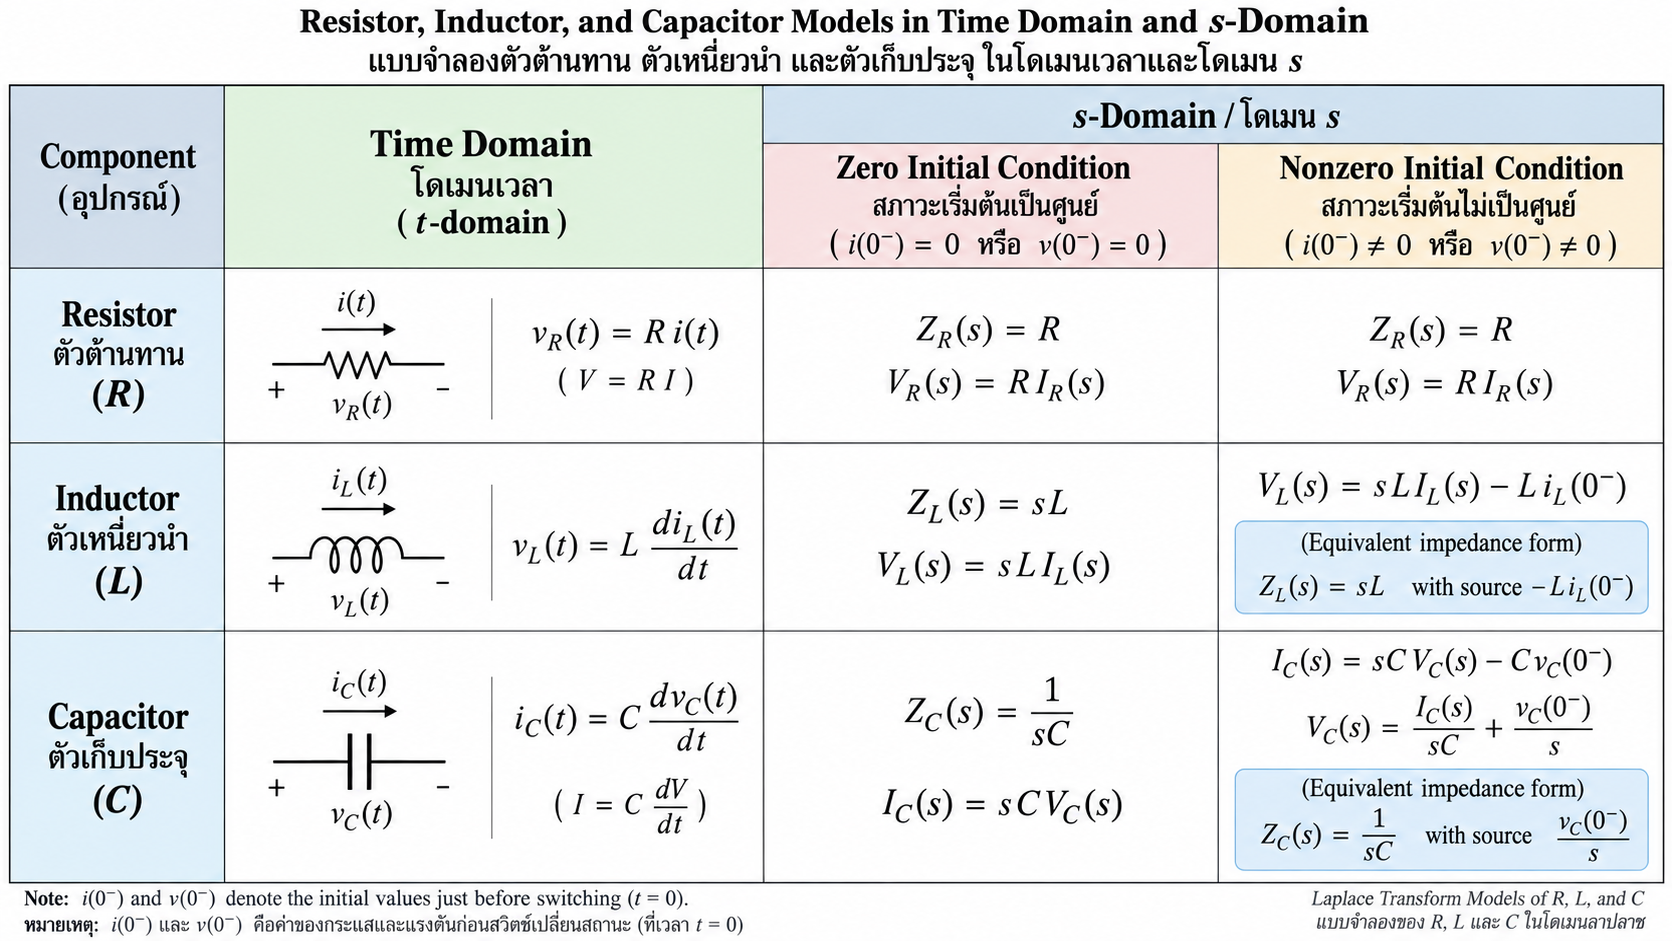
\includegraphics[width=0.8\textwidth]{images/chapter7/figure-03.png}
    \caption{แบบจำลององค์ประกอบ R, L และ C ในโดเมนเวลาและโดเมน $s$}
\end{figure}

\paragraph{7.3.5 แหล่งจ่ายพื้นฐาน}

แรงดันขั้นบันไดขนาด $V_0$

\[
v_s(t)=V_0u(t)
\]

มีลาปลาซ

\[
V_s(s)=\frac{V_0}{s}
\]

กระแสขั้นบันไดขนาด $I_0$

\[
i_s(t)=I_0u(t)
\]

มีลาปลาซ

\[
I_s(s)=\frac{I_0}{s}
\]

หากอินพุตเป็นอิมพัลส์ $\delta(t)$ จะมี $\mathcal{L}\{\delta(t)\}=1$ ซึ่งมีประโยชน์ต่อการนิยาม impulse response และ transfer function แต่ในบทนี้จะเน้นแหล่งขั้นบันไดซึ่งสัมพันธ์กับการเปิดสวิตช์แหล่ง DC มากที่สุด

\paragraph{7.3.6 กระบวนการวิเคราะห์วงจรด้วยลาปลาซแบบ 9 ขั้น}

\begin{enumerate}
    \item \textbf{วิเคราะห์วงจรก่อนสวิตช์} เพื่อหา $v_C(0^-)$ และ $i_L(0^-)$
    \item \textbf{ใช้ความต่อเนื่อง} หา $v_C(0^+)$ และ $i_L(0^+)$
    \item \textbf{วาดวงจรหลังสวิตช์} และกำหนดตัวแปรที่ต้องการหา
    \item \textbf{แปลงแหล่งจ่ายและองค์ประกอบ} ไปเป็นโดเมน $s$
    \item \textbf{คงผลของ initial conditions} ไว้อย่างถูกต้อง
    \item \textbf{ใช้ KVL/KCL หรือวิธีโหนด/เมช} กับวงจรในโดเมน $s$
    \item \textbf{แก้สมการพีชคณิต} เพื่อหา $V(s)$ หรือ $I(s)$
    \item \textbf{แยกเศษส่วนย่อยและหาลาปลาซผกผัน} เพื่อกลับสู่เวลา
    \item \textbf{ตรวจสอบ} ค่า $t=0^+$, $t\rightarrow\infty$, หน่วย และทิศทางทางกายภาพ
\end{enumerate}

% [รูปที่ 4: ขั้นตอน 9 ขั้นในการวิเคราะห์วงจรสวิตช์ด้วยลาปลาซ]
% ประเภทภาพ: Flowchart
% ตำแหน่งที่แนะนำ: หัวข้อ 7.3.6
% วัตถุประสงค์การเรียนรู้: ใช้เป็น checklist ระหว่างแก้โจทย์และลดข้อผิดพลาดเรื่อง initial conditions
% คำอธิบายภาพ: ผังงานหมายเลข 1–9 เริ่มจากวงจร $t<0$ ไปจนถึงการตรวจสอบคำตอบ พร้อมจุดตัดสินใจว่า initial conditions เป็นศูนย์หรือไม่ ถ้าไม่เป็นศูนย์ให้เพิ่มเทอม/แหล่งสมมูล
% องค์ประกอบที่ต้องมี: กล่อง 9 ขั้น ลูกศร จุด decision diamond และกล่อง check final answer
% ข้อความหรือป้ายกำกับ: “Find $v_C(0^-),i_L(0^-)$”, “Transform to $s$ domain”, “Include Initial Conditions”, “Solve”, “Inverse Laplace”, “Verify”
% ภาษาของป้ายกำกับ: ไทยและอังกฤษ
% สัดส่วนภาพ: 16:9
% Image Generation Prompt: Nine-step engineering flowchart for solving switched electrical circuits with Laplace transforms. Steps: analyze t<0 circuit, find capacitor voltage and inductor current initial conditions, apply continuity at 0+, draw t>0 circuit, transform sources and RLC elements to s-domain, include nonzero initial-condition terms, apply KVL/KCL or nodal/mesh analysis, solve algebraic V(s)/I(s), perform inverse Laplace, and verify initial/final values and units. Include a decision diamond for zero versus nonzero initial conditions. Clean white background, bilingual Thai-English labels, vector textbook style, 16:9.
% Graph Generation Prompt: Not applicable.
% Alt Text: ผังงานเก้าขั้นสำหรับแก้ปัญหาวงจรสวิตช์ด้วยการแปลงลาปลาซ

\begin{figure}[htbp]
    \centering
    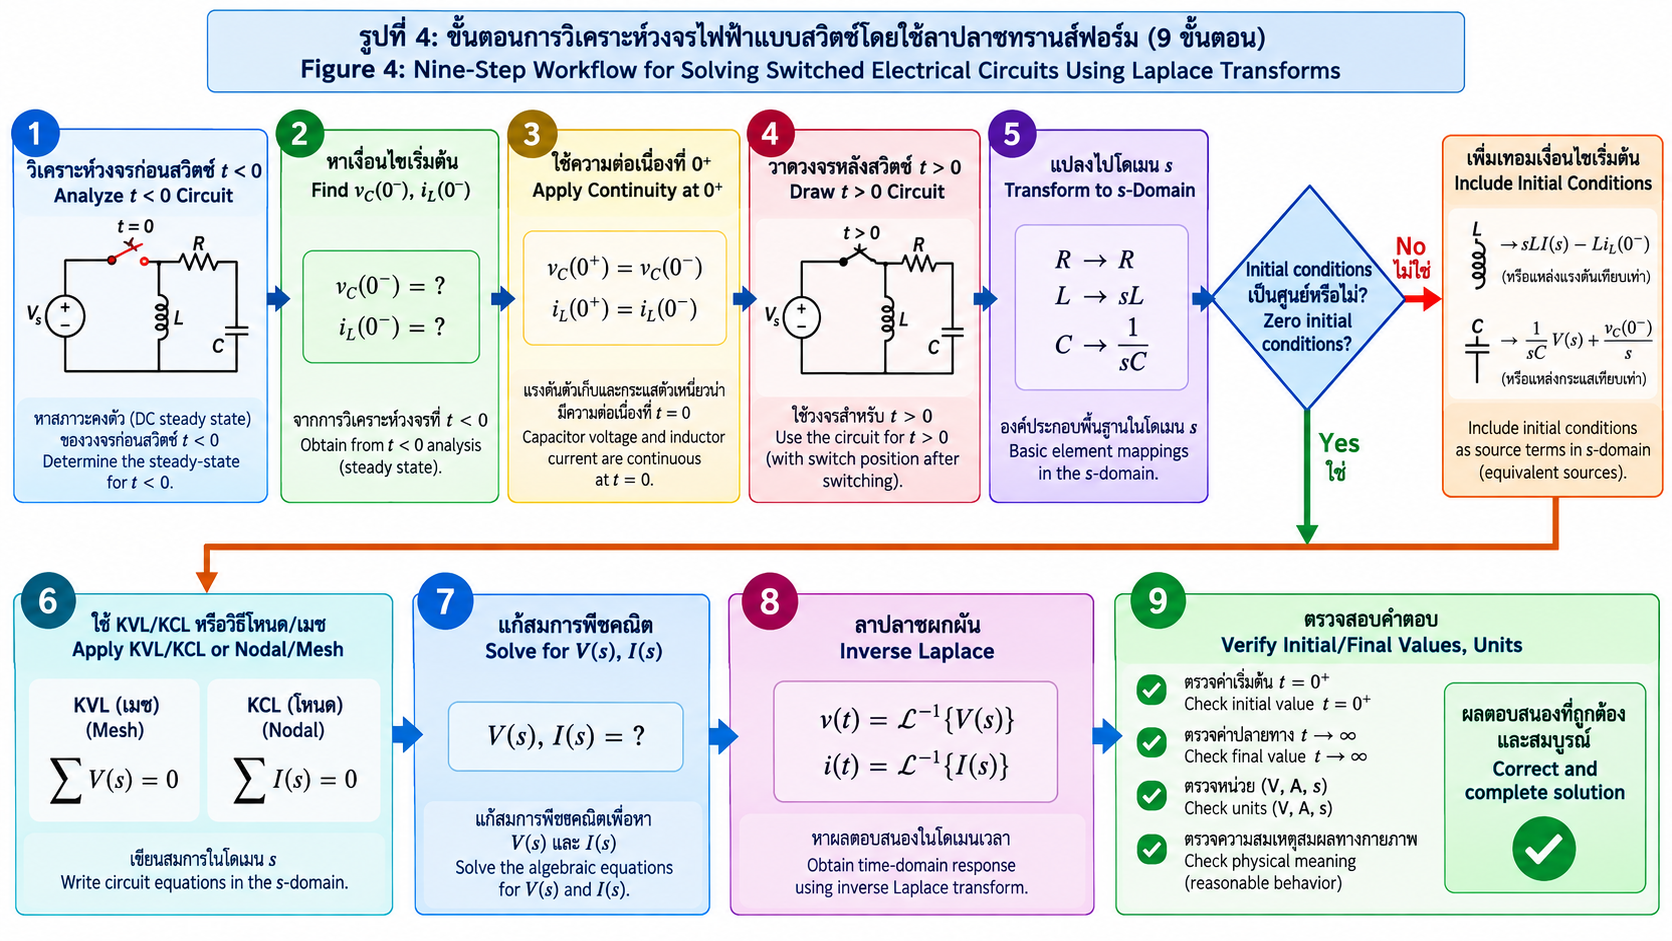
\includegraphics[width=0.8\textwidth]{images/chapter7/figure-04.png}
    \caption{ขั้นตอน 9 ขั้นในการวิเคราะห์วงจรสวิตช์ด้วยลาปลาซ}
\end{figure}

\par\noindent\rule{\textwidth}{0.4pt}\par

\subsubsection{7.4 อิมพีแดนซ์ในโดเมนลาปลาซ}

เมื่อสภาวะเริ่มต้นเป็นศูนย์ วงจรเชิงเส้นที่ประกอบด้วย $R,L,C$ สามารถวิเคราะห์ด้วยกฎพีชคณิตคล้ายวงจรเฟสเซอร์ แต่ตัวแปรคือ $s$ แทน $j\omega$

\[
Z_R(s)=R
\]

\[
Z_L(s)=sL
\]

\[
Z_C(s)=\frac{1}{sC}
\]

สำหรับการต่ออนุกรม

\[
Z_{eq}(s)=Z_1(s)+Z_2(s)+\cdots
\]

สำหรับการต่อขนานนิยมใช้อะแดมิตแตนซ์

\[
Y_{eq}(s)=\frac{1}{Z_{eq}(s)}=Y_1(s)+Y_2(s)+\cdots
\]

ตัวอย่างเช่น RLC อนุกรม

\[
Z_{RLC}(s)=R+sL+\frac{1}{sC}
\]

และเมื่อใช้แหล่งแรงดัน $V_s(s)$ กระแสคือ

\[
I(s)=\frac{V_s(s)}{R+sL+\frac{1}{sC}}
\]

คูณทั้งเศษและส่วนด้วย $sC$

\[
I(s)=\frac{sC\,V_s(s)}{LCs^2+RCs+1}
\]

รูปพหุนาม $LCs^2+RCs+1$ แสดงให้เห็นทันทีว่าวงจรเป็นระบบอันดับสอง และรากของพหุนามนี้สัมพันธ์กับรูปแบบการตอบสนองชั่วครู่

\paragraph{7.4.1 ความแตกต่างระหว่าง $s$-domain impedance กับ phasor impedance}

\begin{table}[htbp]
    \centering
    \small
    \begin{tabularx}{\textwidth}{L{0.19\textwidth} L{0.35\textwidth} Y}
        \hline
        \textbf{ประเด็น} & \textbf{$s$-Domain} & \textbf{Phasor / Sinusoidal Steady State} \\
        \hline
        ตัวแปร & $s=\sigma+j\omega$ & $j\omega$ \\
        จุดประสงค์ & วิเคราะห์ transient + forced response และ initial conditions & วิเคราะห์ steady-state sinusoidal response \\
        ตัวเหนี่ยวนำ & $sL$ เมื่อ IC เป็นศูนย์ & $j\omega L$ \\
        ตัวเก็บประจุ & $1/(sC)$ เมื่อ IC เป็นศูนย์ & $1/(j\omega C)$ \\
        อินพุต & รองรับ step, impulse, exponential, sinusoid ฯลฯ & เน้น sinusoid ที่ความถี่เดียว \\
        สภาวะเริ่มต้น & รวมได้โดยตรงผ่านสมบัติ Laplace & โดยทั่วไปถือว่าผ่าน transient แล้ว \\
        \hline
    \end{tabularx}
\end{table}

ดังนั้นการแทน $s=j\omega$ เป็นเพียงกรณีพิเศษบนแกนจินตภาพที่ใช้ศึกษาการตอบสนองความถี่ ไม่ควรถือว่า phasor analysis และ Laplace analysis เป็นวิธีเดียวกันทุกประการ

\par\noindent\rule{\textwidth}{0.4pt}\par

\subsubsection{7.5 การวิเคราะห์วงจร RC ด้วยการแปลงลาปลาซ}

วงจร RC เป็นระบบอันดับหนึ่งที่เหมาะสำหรับทำความเข้าใจความสัมพันธ์ระหว่างสมการเชิงอนุพันธ์ การแปลงลาปลาซ ค่าคงตัวเวลา โพล และรูปทรงการตอบสนอง

\paragraph{7.5.1 วงจร RC รับแรงดันขั้นบันไดและมีสภาวะเริ่มต้นเป็นศูนย์}

พิจารณาวงจร RC อนุกรม รับอินพุต

\[
v_s(t)=V_0u(t)
\]

และกำหนด $v_C(0^-)=0$ ต้องการหา $v_C(t)$

สมการเวลา

\[
RC\frac{dv_C(t)}{dt}+v_C(t)=V_0u(t)
\]

แปลงลาปลาซ

\[
RC\left[sV_C(s)-v_C(0^-)\right]+V_C(s)=\frac{V_0}{s}
\]

เมื่อ $v_C(0^-)=0$

\[
(RCs+1)V_C(s)=\frac{V_0}{s}
\]

ดังนั้น

\[
V_C(s)=\frac{V_0}{s(RCs+1)}
\]

เขียนด้วย $\tau=RC$

\[
V_C(s)=\frac{V_0}{s(\tau s+1)}
\]

หรือ

\[
V_C(s)=V_0\left(\frac{1}{s}-\frac{1}{s+1/\tau}\right)
\]

จึงได้

\[
\boxed{v_C(t)=V_0\left(1-e^{-t/RC}\right)u(t)}
\]

กระแส

\[
i(t)=C\frac{dv_C}{dt}=\frac{V_0}{R}e^{-t/RC}u(t)
\]

\textbf{ตรวจสอบเชิงกายภาพ}

\begin{itemize}
    \item ที่ $t=0^+$: $v_C(0^+)=0$ ถูกต้องตามความต่อเนื่อง
    \item ที่ $t\to\infty$: $v_C\to V_0$ เพราะ capacitor ใน steady-state DC มีพฤติกรรมเป็นวงจรเปิด
    \item ที่ $t=0^+$: $i(0^+)=V_0/R$ มากที่สุด
    \item ที่ $t\to\infty$: $i\to0$
\end{itemize}

\paragraph{ตัวอย่างที่ 1: การชาร์จตัวเก็บประจุในวงจร RC — ตัวอย่างเพิ่มเติมเพื่อการเรียนรู้}

ให้ $R=2\,\text{k}\Omega$, $C=100\,\mu\text{F}$ และแหล่งแรงดันขั้นบันได $V_s=10\,\text{V}$ ที่ $t=0$ โดยตัวเก็บประจุยังไม่ประจุ จงหา

\begin{enumerate}
    \item $v_C(t)$
    \item $i(t)$
    \item $v_C$ ที่ $t=0.2\,\text{s}$
    \item เวลาประมาณที่ $v_C$ ถึง $95\%$ ของค่าปลายทาง
\end{enumerate}

\textbf{ขั้นที่ 1 วิเคราะห์ระบบ}\\
เป็นวงจร RC อันดับหนึ่ง รับ step input และ $v_C(0^-)=0$

\textbf{ขั้นที่ 2 กำหนดตัวแปร}\\
เอาต์พุตคือแรงดันคร่อม C และกำหนดกระแสไหลจากแหล่งผ่าน R เข้าสู่ C

\textbf{ขั้นที่ 3 เลือกหลักการ}\\
ใช้

\[
RC\frac{dv_C}{dt}+v_C=V_s
\]

และใช้การแปลงลาปลาซตามที่พัฒนาข้างต้น

\textbf{ขั้นที่ 4 คำนวณค่าคงตัวเวลา}

\[
\tau=RC=(2000)(100\times10^{-6})=0.2\,\text{s}
\]

ดังนั้น

\[
\frac{1}{\tau}=5\,\text{s}^{-1}
\]

\textbf{ขั้นที่ 5 เขียนคำตอบแรงดัน}

\[
\boxed{v_C(t)=10\left(1-e^{-5t}\right)\ \text{V}}
\]

\textbf{ขั้นที่ 6 หาค่ากระแส}

\[
i(t)=\frac{10}{2000}e^{-5t}
\]

\[
\boxed{i(t)=5e^{-5t}\ \text{mA}}
\]

\textbf{ขั้นที่ 7 คำนวณที่ $t=0.2\,\text{s}=\tau$}

\[
v_C(0.2)=10(1-e^{-1})
\]

โดย $e^{-1}\approx0.3679$

\[
v_C(0.2)\approx10(0.6321)=6.321\,\text{V}
\]

\textbf{ขั้นที่ 8 เวลาถึง $95\%$}

กำหนด

\[
0.95V_s=V_s(1-e^{-t/\tau})
\]

จึงได้

\[
e^{-t/\tau}=0.05
\]

\[
t=-\tau\ln(0.05)
\]

\[
t=(0.2)(2.9957)\approx0.599\,\text{s}
\]

หรือประมาณ $3\tau$

\textbf{ขั้นที่ 9 ตรวจสอบความสมเหตุสมผล}\\
ที่ $t=0$ แรงดัน C เป็นศูนย์ และที่เวลานานมากเข้าใกล้ 10 V ส่วนกระแสเริ่มที่ 5 mA แล้วลดลงสู่ศูนย์ ซึ่งสอดคล้องกับพฤติกรรมการชาร์จของ capacitor

% [รูปที่ 5: การตอบสนองขั้นบันไดของวงจร RC]
% ประเภทภาพ: Graph
% ตำแหน่งที่แนะนำ: หลังตัวอย่างที่ 1
% วัตถุประสงค์การเรียนรู้: เชื่อมสมการ $v_C(t)=V_0(1-e^{-t/\tau})$ กับความหมายของ time constant
% คำอธิบายภาพ: กราฟ $v_C(t)$ เพิ่มจาก 0 ไปยัง $V_0$ และกราฟ $i(t)$ ลดจาก $V_0/R$ ไปยัง 0 พร้อมเส้นประที่ $t=\tau,3\tau,5\tau$ และป้าย 63.2%, 95.0%, 99.3%
% องค์ประกอบที่ต้องมี: แกนเวลา หน่วยวินาที เส้น $v_C/V_0$ เส้น $i/(V_0/R)$ จุด $\tau$, $3\tau$, $5\tau$
% ข้อความหรือป้ายกำกับ: “Charging Voltage”, “Charging Current”, “Time Constant $\tau=RC$”
% ภาษาของป้ายกำกับ: ไทยและอังกฤษ
% สัดส่วนภาพ: 16:9
% Image Generation Prompt: Engineering mathematics graph for a first-order RC step response. Show normalized capacitor voltage v_C/V0 = 1-exp(-t/tau) rising from 0 to 1 and normalized current i/(V0/R)=exp(-t/tau) decaying from 1 to 0. Mark t=tau, 3tau and 5tau with 63.2%, 95.0% and about 99.3% response levels. Precise axes, white background, bilingual Thai-English annotations, clean vector textbook style, 16:9.
% Graph Generation Prompt: Plot $v_C/V_0=1-e^{-t/\tau}$ and $i/(V_0/R)=e^{-t/\tau}$ for $0\le t\le5\tau$. x-axis: $t/\tau$ from 0 to 5. y-axis: normalized amplitude from 0 to 1.05. Mark $(1,0.632)$, $(3,0.950)$ and $(5,0.993)$ on the voltage curve.
% Alt Text: กราฟแรงดันตัวเก็บประจุเพิ่มแบบเอ็กซ์โพเนนเชียลและกระแสลดแบบเอ็กซ์โพเนนเชียล พร้อมจุดหนึ่ง สาม และห้าค่าคงตัวเวลา

\begin{figure}[htbp]
    \centering
    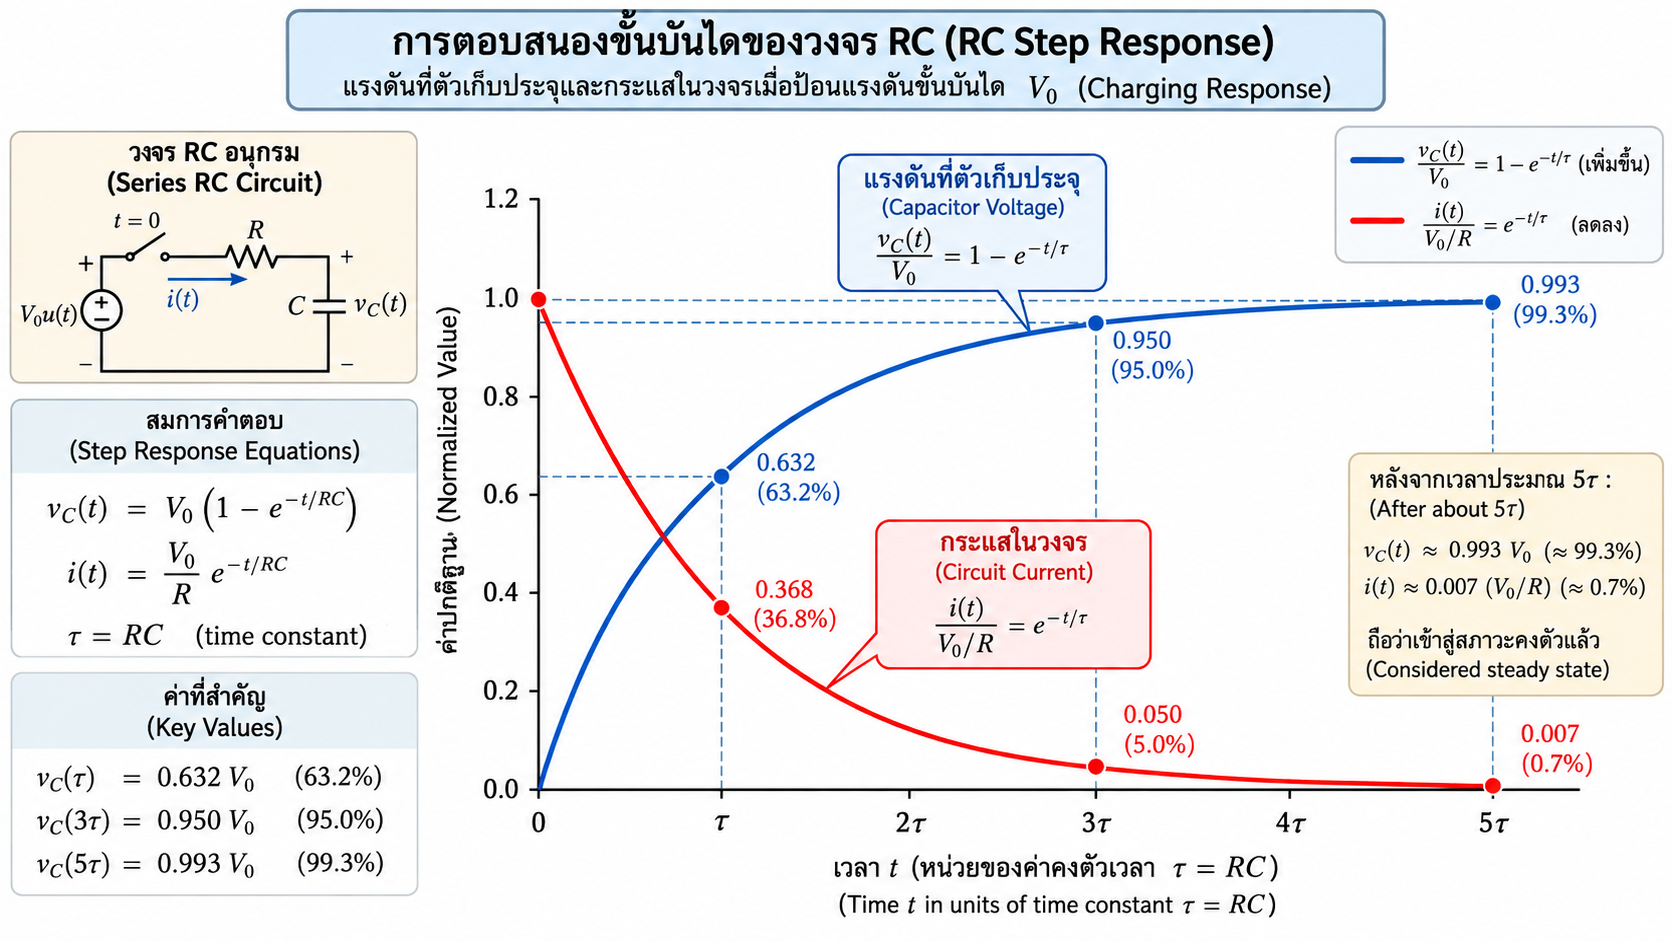
\includegraphics[width=0.8\textwidth]{images/chapter7/figure-05.png}
    \caption{การตอบสนองขั้นบันไดของวงจร RC}
\end{figure}

\paragraph{7.5.2 RC ที่มีแรงดันเริ่มต้นไม่เป็นศูนย์}

กรณีทั่วไปเมื่อหลังสวิตช์วงจรมีค่า Thevenin เทียบเท่า $V_{\text{th}}$ และ $R_{\text{th}}$ มองจากขั้ว capacitor ค่าปลายทางคือ $V_f=V_{\text{th}}$ และค่าคงตัวเวลา

\[
\tau=R_{\text{th}}C
\]

รูปคำตอบสามารถเขียนอย่างมีประสิทธิภาพได้เป็น

\[
\boxed{v_C(t)=V_f+[v_C(0^+)-V_f]e^{-t/\tau}}
\]

สมการนี้เป็นรูป time-domain ที่มีประโยชน์มาก แต่การแปลงลาปลาซยังคงสำคัญเมื่อวงจรมีหลายแหล่งหรือเมื่อไม่สามารถเห็น $V_f$ และ $R_{\text{th}}$ ได้ง่าย

\paragraph{ตัวอย่างที่ 2: วงจร RC ที่มีประจุเริ่มต้น — ตัวอย่างเพิ่มเติมเพื่อการเรียนรู้}

ตัวเก็บประจุ $C=50\,\mu\text{F}$ มีแรงดันเริ่มต้น $v_C(0^-)=4\,\text{V}$ ที่ $t=0$ ถูกต่อผ่าน $R=4\,\text{k}\Omega$ เข้ากับแหล่ง DC 12 V จงหา $v_C(t)$ และกระแสเริ่มต้น

\textbf{1. วิเคราะห์สภาวะเริ่มต้น}

\[
v_C(0^+)=v_C(0^-)=4\,\text{V}
\]

\textbf{2. ค่าปลายทาง}

ที่ $t\to\infty$ กระแสเป็นศูนย์ จึงไม่มีแรงดันตกคร่อม R

\[
V_f=12\,\text{V}
\]

\textbf{3. ค่าคงตัวเวลา}

\[
\tau=RC=(4000)(50\times10^{-6})=0.2\,\text{s}
\]

\textbf{4. เขียนคำตอบ}

\[
v_C(t)=12+(4-12)e^{-t/0.2}
\]

\[
\boxed{v_C(t)=12-8e^{-5t}\ \text{V}}
\]

\textbf{5. กระแสเริ่มต้น}

\[
i(0^+)=\frac{12-4}{4000}=2\,\text{mA}
\]

\textbf{6. ตรวจสอบ}\\
ที่ $t=0$: $12-8=4$ V และที่ $t\to\infty$: $v_C\to12$ V ถูกต้อง

\paragraph{7.5.3 ฟังก์ชันถ่ายโอนของวงจร RC}

เมื่อสภาวะเริ่มต้นเป็นศูนย์ ฟังก์ชันถ่ายโอนจาก $v_s$ ไปยัง $v_C$ คือ

\[
H_{LP}(s)=\frac{V_C(s)}{V_s(s)}=\frac{1}{RCs+1}
\]

เรียกว่าโครงสร้าง low-pass อันดับหนึ่ง มีโพลที่

\[
p=-\frac{1}{RC}
\]

ถ้าเลือกแรงดันตัวต้านทานเป็นเอาต์พุต

\[
H_{HP}(s)=\frac{V_R(s)}{V_s(s)}=\frac{RCs}{RCs+1}
\]

มีซีโรที่ $s=0$ และโพลเดียวกันที่ $-1/(RC)$ รูปสองสมการนี้แสดงให้เห็นว่า \textbf{วงจรเดียวกันแต่เลือกเอาต์พุตต่างกัน สามารถมี zero structure ต่างกันได้}

\par\noindent\rule{\textwidth}{0.4pt}\par

\subsubsection{7.6 การวิเคราะห์วงจร RL ด้วยการแปลงลาปลาซ}

\paragraph{7.6.1 การตอบสนองขั้นบันไดของวงจร RL}

พิจารณา $R$ และ $L$ อนุกรม รับแหล่งแรงดัน $V_0u(t)$ และ $i_L(0^-)=0$

สมการเวลา

\[
L\frac{di(t)}{dt}+Ri(t)=V_0u(t)
\]

แปลงลาปลาซ

\[
L[sI(s)-i(0^-)]+RI(s)=\frac{V_0}{s}
\]

เมื่อ $i(0^-)=0$

\[
(sL+R)I(s)=\frac{V_0}{s}
\]

ดังนั้น

\[
I(s)=\frac{V_0}{s(sL+R)}
\]

จัดรูปด้วย $\tau=L/R$

\[
I(s)=\frac{V_0/R}{s(\tau s+1)}
\]

ลาปลาซผกผัน

\[
\boxed{i(t)=\frac{V_0}{R}\left(1-e^{-tR/L}\right)u(t)}
\]

หรือ

\[
\boxed{i(t)=I_f\left(1-e^{-t/\tau}\right)}
\]

โดย

\[
I_f=\frac{V_0}{R},\qquad \tau=\frac{L}{R}
\]

แรงดันตัวเหนี่ยวนำ

\[
v_L(t)=L\frac{di}{dt}=V_0e^{-tR/L}
\]

แรงดันตัวต้านทาน

\[
v_R(t)=Ri(t)=V_0\left(1-e^{-tR/L}\right)
\]

จึงเห็นการถ่ายโอนแรงดันจากตัวเหนี่ยวนำไปยังตัวต้านทานตามเวลา โดย KVL ยังคงเป็นจริงทุกขณะ

\paragraph{ตัวอย่างที่ 3: การสร้างกระแสในวงจร RL — ตัวอย่างเพิ่มเติมเพื่อการเรียนรู้}

ให้ $V_s=24\,\text{V}$, $R=12\,\Omega$, $L=0.6\,\text{H}$ และ $i_L(0^-)=0$ จงหา $i(t)$, $v_L(t)$ และเวลาที่กระแสถึง $90\%$ ของค่าปลายทาง

\textbf{ขั้นที่ 1 แบบจำลอง}

\[
L\frac{di}{dt}+Ri=24u(t)
\]

\textbf{ขั้นที่ 2 ค่าคงตัวเวลา}

\[
\tau=\frac{L}{R}=\frac{0.6}{12}=0.05\,\text{s}
\]

\textbf{ขั้นที่ 3 ค่าปลายทาง}

\[
I_f=\frac{24}{12}=2\,\text{A}
\]

\textbf{ขั้นที่ 4 กระแส}

\[
\boxed{i(t)=2\left(1-e^{-20t}\right)\ \text{A}}
\]

\textbf{ขั้นที่ 5 แรงดันตัวเหนี่ยวนำ}

\[
\boxed{v_L(t)=24e^{-20t}\ \text{V}}
\]

\textbf{ขั้นที่ 6 เวลาถึง 90\%}

\[
0.9=1-e^{-t/\tau}
\]

\[
e^{-t/\tau}=0.1
\]

\[
t=-\tau\ln(0.1)=0.05(2.3026)=0.1151\,\text{s}
\]

ดังนั้น

\[
\boxed{t_{90}\approx0.115\,\text{s}}
\]

\textbf{ขั้นที่ 7 ตรวจสอบ}\\
ที่ $t=0^+$ กระแสยังเป็น 0 A แต่แรงดันทั้งหมด 24 V อยู่ที่ L; เมื่อเวลานานมาก L มีพฤติกรรมเป็นลัดวงจรใน DC กระแสจึงเข้าใกล้ 2 A และ $v_L\to0$

% [รูปที่ 6: การตอบสนองขั้นบันไดของวงจร RL]
% ประเภทภาพ: Graph
% ตำแหน่งที่แนะนำ: หลังตัวอย่างที่ 3
% วัตถุประสงค์การเรียนรู้: เชื่อมการเพิ่มของกระแสกับการลดลงของแรงดันตัวเหนี่ยวนำ
% คำอธิบายภาพ: แสดง $i/I_f=1-e^{-t/\tau}$ และ $v_L/V_0=e^{-t/\tau}$ ในกราฟเดียว พร้อมจุดที่ $t=\tau$
% องค์ประกอบที่ต้องมี: แกน $t/\tau$, เส้น normalized current และ normalized inductor voltage, เส้นประ $t=\tau$
% ข้อความหรือป้ายกำกับ: “Current Build-up”, “Inductor Voltage Decay”, “$\tau=L/R$”
% ภาษาของป้ายกำกับ: ไทยและอังกฤษ
% สัดส่วนภาพ: 16:9
% Image Generation Prompt: Clean engineering graph of an RL step response. Plot normalized current i/If = 1-exp(-t/tau) rising from 0 to 1 and normalized inductor voltage vL/V0 = exp(-t/tau) decaying from 1 to 0. Mark t=tau and the 63.2% current point. White background, precise axes, bilingual Thai-English labels, vector textbook style, 16:9.
% Graph Generation Prompt: Plot $i/I_f=1-e^{-t/\tau}$ and $v_L/V_0=e^{-t/\tau}$ for $0\le t\le5\tau$, with x-axis $t/\tau$ and normalized y-axis 0 to 1.05.
% Alt Text: กราฟแสดงกระแส RL เพิ่มขึ้นและแรงดันตัวเหนี่ยวนำลดลงด้วยค่าคงตัวเวลาเดียวกัน

\begin{figure}[htbp]
    \centering
    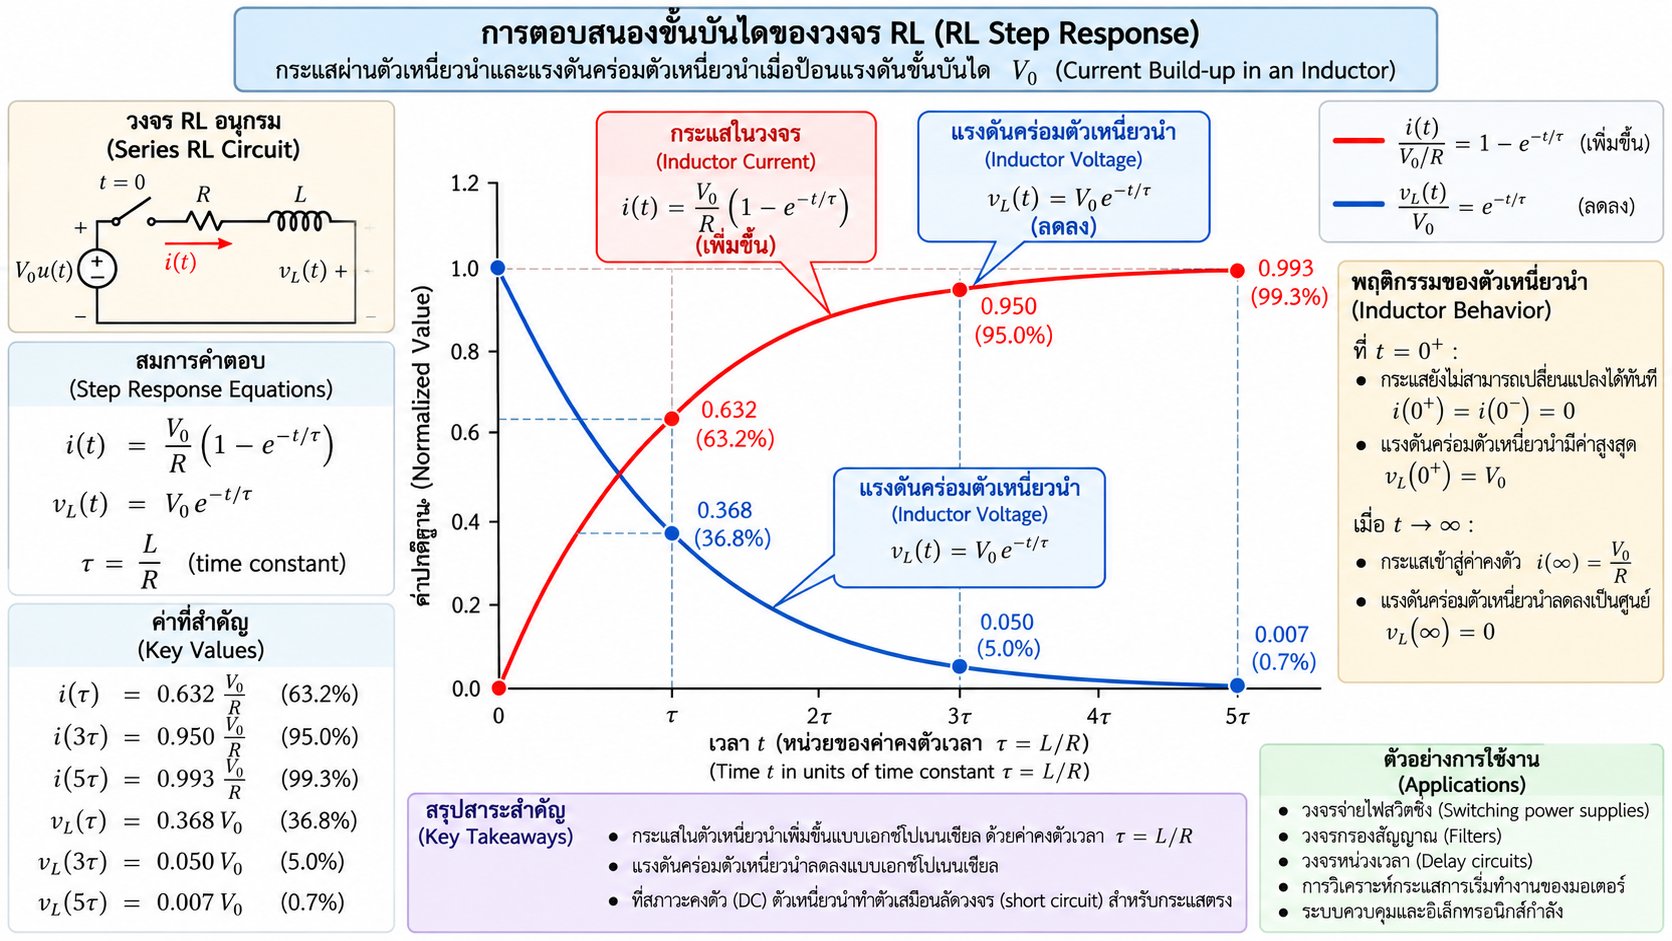
\includegraphics[width=0.8\textwidth]{images/chapter7/figure-06.png}
    \caption{การตอบสนองขั้นบันไดของวงจร RL}
\end{figure}

\paragraph{7.6.2 RL ที่มีกระแสเริ่มต้นไม่เป็นศูนย์}

หากหลังสวิตช์วงจรมองจากตัวเหนี่ยวนำมีค่าเทียบเท่า $V_{\text{th}}$ และ $R_{\text{th}}$ กระแสมีรูปทั่วไป

\[
\boxed{i_L(t)=I_f+[i_L(0^+)-I_f]e^{-t/\tau}}
\]

โดย

\[
I_f=\frac{V_{\text{th}}}{R_{\text{th}}},\qquad \tau=\frac{L}{R_{\text{th}}}
\]

กรณี source-free RL ที่ $I_f=0$

\[
\boxed{i_L(t)=I_0e^{-tR/L}}
\]

พลังงานที่เก็บใน L จะค่อย ๆ ถูกสลายผ่าน R

\[
W_L(t)=\frac{1}{2}Li_L^2(t)
\]

ดังนั้นพลังงานลดตาม $e^{-2t/\tau}$ ซึ่งเร็วกว่าแอมพลิจูดกระแสในเชิงเลขชี้กำลังสองเท่า

\par\noindent\rule{\textwidth}{0.4pt}\par

\subsubsection{7.7 การวิเคราะห์วงจร RLC ด้วยการแปลงลาปลาซ}

วงจร RLC มีองค์ประกอบเก็บพลังงานสองชนิด จึงมีสมการอันดับสองและสามารถแสดงการสั่นได้ การแปลงลาปลาซทำให้การหาคำตอบเป็นการวิเคราะห์รากของพหุนามอันดับสอง

\paragraph{7.7.1 ฟังก์ชันในโดเมน $s$ สำหรับ RLC อนุกรม}

จาก

\[
LC\frac{d^2v_C}{dt^2}+RC\frac{dv_C}{dt}+v_C=v_s(t)
\]

เมื่อสภาวะเริ่มต้นเป็นศูนย์

\[
LCs^2V_C(s)+RCsV_C(s)+V_C(s)=V_s(s)
\]

ดังนั้น

\[
\boxed{\frac{V_C(s)}{V_s(s)}=\frac{1}{LCs^2+RCs+1}}
\]

หารด้วย $LC$

\[
\boxed{H(s)=\frac{\omega_n^2}{s^2+2\zeta\omega_ns+\omega_n^2}}
\]

โดย

\[
\omega_n=\frac{1}{\sqrt{LC}},\qquad 2\zeta\omega_n=\frac{R}{L}
\]

รากของสมการลักษณะเฉพาะ

\[
s^2+2\zeta\omega_ns+\omega_n^2=0
\]

คือ

\[
s_{1,2}=-\zeta\omega_n\pm\omega_n\sqrt{\zeta^2-1}
\]

หรือเขียนด้วย $\alpha=R/(2L)$

\[
s_{1,2}=-\alpha\pm\sqrt{\alpha^2-\omega_n^2}
\]

\paragraph{7.7.2 กรณี underdamped}

เมื่อ $\zeta<1$

\[
s_{1,2}=-\zeta\omega_n\pm j\omega_d
\]

โดย

\[
\omega_d=\omega_n\sqrt{1-\zeta^2}
\]

จึงมีองค์ประกอบเวลาในรูป

\[
e^{-\zeta\omega_nt}\cos\omega_dt,\qquad e^{-\zeta\omega_nt}\sin\omega_dt
\]

ส่วนจริงลบของโพลทำให้ซองการสั่นลดลง ส่วนจินตภาพกำหนดความถี่การสั่นที่สังเกตได้

\paragraph{7.7.3 กรณี critically damped}

เมื่อ $\zeta=1$ มีโพลซ้ำ

\[
s_1=s_2=-\omega_n
\]

คำตอบธรรมชาติมีรูป

\[
y_n(t)=(A+Bt)e^{-\omega_nt}
\]

กรณีนี้ไม่สั่นและเป็นขอบเขตระหว่างระบบที่สั่นกับไม่สั่น

\paragraph{7.7.4 กรณี overdamped}

เมื่อ $\zeta>1$ จะมีโพลจริงลบสองตัว

\[
s_1<0,\qquad s_2<0
\]

คำตอบเป็นผลรวมของเอ็กซ์โพเนนเชียลสองพจน์

\[
y_n(t)=A e^{s_1t}+B e^{s_2t}
\]

โพลที่อยู่ใกล้แกนจินตภาพมากกว่า หรือมีค่าจริงลบน้อยกว่า มักมีการลดทอนช้ากว่าและมีอิทธิพลต่อช่วงท้ายของ transient มากกว่า

\paragraph{ตัวอย่างที่ 4: วิเคราะห์ชนิดการหน่วงของวงจร RLC — ตัวอย่างเพิ่มเติมเพื่อการเรียนรู้}

ให้วงจร RLC อนุกรมมี

\[
L=0.5\,\text{H},\qquad C=200\,\mu\text{F}
\]

จงหา $\omega_n$, $R_{\text{crit}}$ และจำแนกลักษณะการตอบสนองเมื่อ $R=20\,\Omega$, $100\,\Omega$ และ $200\,\Omega$

\textbf{ขั้นที่ 1 คำนวณความถี่ธรรมชาติ}

\[
LC=(0.5)(200\times10^{-6})=1.0\times10^{-4}
\]

\[
\omega_n=\frac{1}{\sqrt{10^{-4}}}=100\,\text{rad/s}
\]

\textbf{ขั้นที่ 2 คำนวณความต้านทานวิกฤต}

\[
R_{\text{crit}}=2\sqrt{\frac{L}{C}}
\]

\[
=2\sqrt{\frac{0.5}{200\times10^{-6}}}
\]

\[
=2\sqrt{2500}=100\,\Omega
\]

ดังนั้น

\begin{itemize}
    \item $R=20\,\Omega<R_{\text{crit}}$ $\to$ \textbf{underdamped}
    \item $R=100\,\Omega=R_{\text{crit}}$ $\to$ \textbf{critically damped}
    \item $R=200\,\Omega>R_{\text{crit}}$ $\to$ \textbf{overdamped}
\end{itemize}

สำหรับ $R=20\,\Omega$

\[
\alpha=\frac{R}{2L}=\frac{20}{1}=20\,\text{s}^{-1}
\]

\[
\zeta=\frac{20}{100}=0.2
\]

\[
\omega_d=100\sqrt{1-0.2^2}\approx97.98\,\text{rad/s}
\]

จึงคาดว่าจะเห็นการสั่นที่ซองลดลงประมาณ $e^{-20t}$

\textbf{ตรวจสอบความหมาย:} การเพิ่ม R ทำให้สูญเสียพลังงานมากขึ้นต่อรอบและเพิ่มการหน่วง จึงเปลี่ยนระบบจาก underdamped ไปสู่ critically damped และ overdamped ตามลำดับ

% [รูปที่ 7: เปรียบเทียบการตอบสนอง RLC แบบ underdamped, critically damped และ overdamped]
% ประเภทภาพ: Graph
% ตำแหน่งที่แนะนำ: หลังตัวอย่างที่ 4
% วัตถุประสงค์การเรียนรู้: เชื่อมค่า $R$, $\zeta$ และตำแหน่งโพลกับรูปกราฟเวลา
% คำอธิบายภาพ: แสดง step responses สามเส้นของระบบอันดับสอง normalized โดย underdamped มี overshoot และการสั่นลดลง critically damped ขึ้นถึงค่าปลายทางเร็วโดยไม่สั่น และ overdamped ช้ากว่าโดยไม่สั่น
% องค์ประกอบที่ต้องมี: แกน normalized time $\omega_nt$, normalized output, เส้นสามชนิด, เส้นค่าปลายทาง 1.0 และภาพ inset แสดงตำแหน่งโพล
% ข้อความหรือป้ายกำกับ: “Underdamped $\zeta<1$”, “Critical $\zeta=1$”, “Overdamped $\zeta>1$”, “Pole Locations”
% ภาษาของป้ายกำกับ: ไทยและอังกฤษ
% สัดส่วนภาพ: 16:9
% Image Generation Prompt: Engineering textbook graph comparing normalized second-order RLC step responses for underdamped, critically damped, and overdamped cases. Underdamped curve has decaying oscillation and overshoot, critical curve reaches the final value quickly without oscillation, overdamped curve is slower without oscillation. Include a small inset s-plane showing corresponding pole locations. Precise axes, white background, bilingual Thai-English labels, vector style, 16:9.
% Graph Generation Prompt: Plot normalized standard second-order step responses for representative damping ratios $\zeta=0.2$, $1.0$, and $2.0$ versus normalized time $\omega_nt$ from 0 to 10. Mark final value 1.0. Include pole inset at $-\zeta\omega_n\pm j\omega_n\sqrt{1-\zeta^2}$ for $\zeta<1$ and real negative poles for $\zeta\ge1$.
% Alt Text: กราฟเปรียบเทียบการตอบสนองอันดับสองสามชนิดและตำแหน่งโพลที่สอดคล้องกัน

\begin{figure}[htbp]
    \centering
    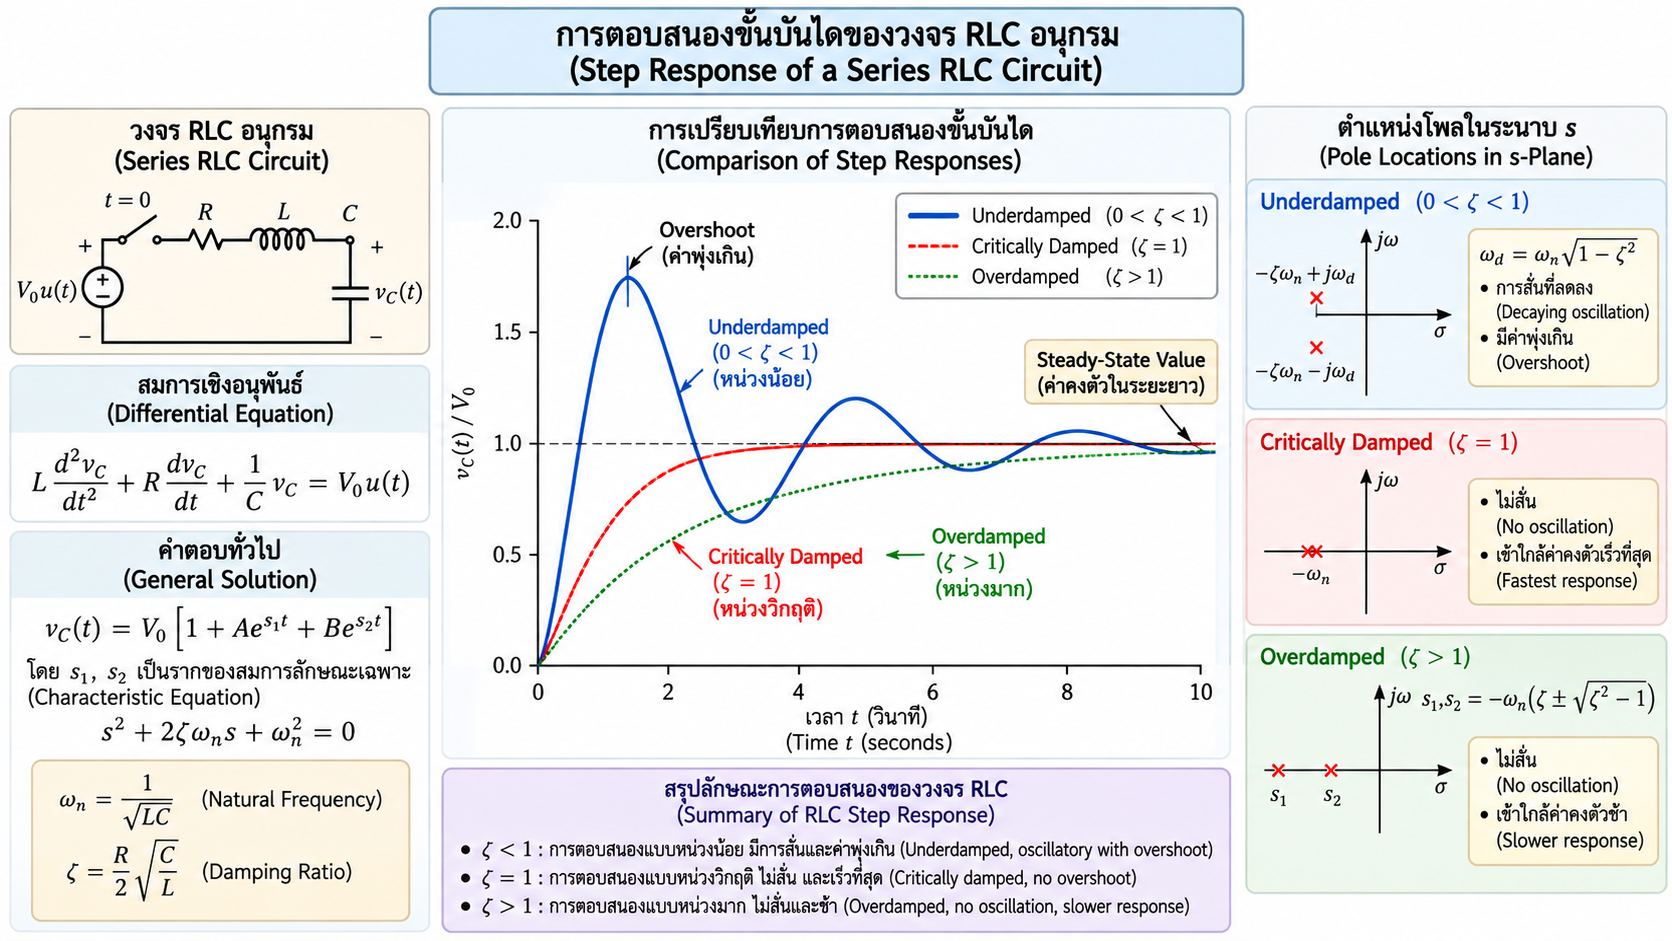
\includegraphics[width=0.8\textwidth]{images/chapter7/figure-07.png}
    \caption{เปรียบเทียบการตอบสนอง RLC แบบ underdamped, critically damped และ overdamped}
\end{figure}

\paragraph{ตัวอย่างที่ 5: หาการตอบสนองขั้นบันไดของ RLC แบบ underdamped — ตัวอย่างเพิ่มเติมเพื่อการเรียนรู้}

ใช้วงจรจากตัวอย่างที่ 4 โดย $R=20\,\Omega$, $L=0.5\,\text{H}$, $C=200\,\mu\text{F}$ รับ step $v_s(t)=10u(t)$ V และสภาวะเริ่มต้นเป็นศูนย์ จงหา $v_C(t)$

จากตัวอย่างที่ 4

\[
\omega_n=100\,\text{rad/s},\qquad \zeta=0.2,\qquad \omega_d\approx97.98\,\text{rad/s}
\]

ฟังก์ชันถ่ายโอนคือ

\[
H(s)=\frac{10000}{s^2+40s+10000}
\]

อินพุต

\[
V_s(s)=\frac{10}{s}
\]

ดังนั้น

\[
V_C(s)=\frac{100000}{s(s^2+40s+10000)}
\]

เขียนส่วนกำลังสองเป็น

\[
s^2+40s+10000=(s+20)^2+9600
\]

และ

\[
\sqrt{9600}\approx97.98
\]

สำหรับ step response ของระบบอันดับสอง underdamped ที่ DC gain เท่ากับ 1

\[
v_C(t)=10\left[1-e^{-\zeta\omega_nt}\left(\cos\omega_dt+\frac{\zeta}{\sqrt{1-\zeta^2}}\sin\omega_dt\right)\right]
\]

แทนค่า

\[
\frac{\zeta}{\sqrt{1-\zeta^2}}=\frac{0.2}{\sqrt{0.96}}\approx0.2041
\]

จึงได้

\[
\boxed{v_C(t)=10\left[1-e^{-20t}\left(\cos(97.98t)+0.2041\sin(97.98t)\right)\right]\ \text{V}}
\]

\textbf{ตรวจสอบค่าเริ่มต้น}

ที่ $t=0$

\[
v_C(0)=10[1-(1)(1+0)]=0\,\text{V}
\]

\textbf{ตรวจสอบค่าปลายทาง}

เมื่อ $t\to\infty$, $e^{-20t}\to0$

\[
v_C(\infty)=10\,\text{V}
\]

\textbf{ตีความ:} แรงดัน capacitor จะมี overshoot และการสั่นชั่วครู่ก่อนเข้าสู่ 10 V เนื่องจากมีการแลกเปลี่ยนพลังงานระหว่าง L และ C ขณะที่ R ค่อย ๆ สลายพลังงานและทำให้การสั่นลดลง

\par\noindent\rule{\textwidth}{0.4pt}\par

\subsubsection{7.8 การตอบสนองชั่วครู่และการตอบสนองบังคับ}

การอธิบายการตอบสนองของวงจรให้แม่นยำควรแยกแนวคิดที่คล้ายกันแต่ไม่เหมือนกันออกจากกัน

\paragraph{7.8.1 Natural response และ forced response}

สำหรับระบบเชิงเส้นที่อธิบายด้วยสมการเชิงอนุพันธ์

\[
\text{Total Response}=\text{Natural Response}+\text{Forced Response}
\]

\begin{itemize}
    \item \textbf{Natural response} เกิดจากพลังงานเริ่มต้นและโครงสร้างของระบบ สัมพันธ์กับคำตอบของสมการเอกพันธ์และโพลของระบบ
    \item \textbf{Forced response} เกิดจากอินพุตภายนอกและขึ้นกับรูปของอินพุต
\end{itemize}

ตัวอย่าง RC ที่รับ DC step

\[
v_C(t)=V_f+[V_0-V_f]e^{-t/\tau}
\]

สามารถมองได้ว่า

\begin{itemize}
    \item พจน์ $[V_0-V_f]e^{-t/\tau}$ เป็นองค์ประกอบธรรมชาติที่ลดลงตามโพล $-1/\tau$
    \item พจน์คงที่ $V_f$ เป็นองค์ประกอบที่สอดคล้องกับการบังคับโดยแหล่ง DC ในระยะยาว
\end{itemize}

\paragraph{7.8.2 Zero-input response และ zero-state response}

ในวิชาระบบเชิงเส้นมักแยกอีกแบบหนึ่งว่า

\[
\text{Total Response}=\text{Zero-Input Response}+\text{Zero-State Response}
\]

\begin{itemize}
    \item \textbf{Zero-input response:} อินพุตเป็นศูนย์ แต่มี initial conditions
    \item \textbf{Zero-state response:} initial conditions เป็นศูนย์ แต่มีอินพุต
\end{itemize}

คำสองคู่นี้เกี่ยวข้องกัน แต่ไม่ควรใช้แทนกันโดยไม่พิจารณาบริบท โดยเฉพาะ forced response บางกรณีอาจยังมี transient terms ที่เกิดจากการเริ่มอินพุตที่ $t=0$

\paragraph{7.8.3 Transient response และ steady-state response}

ในทางวิศวกรรม มักเขียน

\[
\text{Total Response}=\text{Transient Response}+\text{Steady-State Response}
\]

สำหรับระบบเสถียรที่รับอินพุตคงที่หรือไซน์ ส่วน transient จะลดลงตามเวลา ส่วน steady-state จะเป็นพฤติกรรมที่เหลืออยู่เมื่อ $t\to\infty$

\textbf{ตัวอย่าง RC step}

\[
v_C(t)=V_0(1-e^{-t/\tau})
\]

\begin{itemize}
    \item transient term: $-V_0e^{-t/\tau}$
    \item steady-state term: $V_0$
\end{itemize}

\textbf{ตัวอย่าง RLC underdamped}\\
transient ประกอบด้วยพจน์ $e^{-\zeta\omega_nt}\sin\omega_dt$ และ $e^{-\zeta\omega_nt}\cos\omega_dt$ ซึ่งค่อย ๆ ลดลงหาก $\zeta>0$

\paragraph{7.8.4 ตารางสรุปแนวคิดการตอบสนอง}

\begin{table}[htbp]
    \centering
    \small
    \setlength{\tabcolsep}{4pt}
    \begin{tabularx}{\textwidth}{L{0.17\textwidth} L{0.18\textwidth} L{0.16\textwidth} L{0.13\textwidth} Y}
        \hline
        \textbf{แนวคิด} & \textbf{เน้นอะไร} & \textbf{เกี่ยวกับ initial condition} & \textbf{เกี่ยวกับ input} & \textbf{ลดลงเสมอหรือไม่} \\
        \hline
        Natural response & โหมดธรรมชาติของระบบ & มีบทบาทสำคัญ & ไม่จำเป็น & ลดลงถ้าโพลมีส่วนจริงลบ \\
        Forced response & ผลจากอินพุต & อาจร่วมกับเงื่อนไขอื่น & มี & ไม่จำเป็น \\
        Zero-input response & พลังงานเริ่มต้น & ใช่ & อินพุตเป็นศูนย์ & ขึ้นกับเสถียรภาพ \\
        Zero-state response & ผลจากอินพุตเมื่อไม่มีพลังงานเริ่มต้น & เป็นศูนย์ & ใช่ & มีทั้ง transient/steady-state ได้ \\
        Transient response & พฤติกรรมช่วงเปลี่ยนผ่าน & อาจเกี่ยวข้อง & อาจเกี่ยวข้อง & สำหรับระบบเสถียรจะลดลง \\
        Steady-state response & พฤติกรรมระยะยาว & ผลเริ่มต้นหายไปในระบบ asymptotically stable & ขึ้นกับอินพุต & คงอยู่ระยะยาว \\
        \hline
    \end{tabularx}
\end{table}

\par\noindent\rule{\textwidth}{0.4pt}\par

\subsubsection{7.9 ฟังก์ชันถ่ายโอนของวงจรไฟฟ้า}

\paragraph{7.9.1 นิยาม}

สำหรับระบบเชิงเส้นไม่แปรตามเวลา (LTI) ที่มีอินพุต $x(t)$ และเอาต์พุต $y(t)$ ฟังก์ชันถ่ายโอนนิยามเป็น

\[
\boxed{G(s)=\frac{Y(s)}{X(s)}\bigg|_{\text{initial conditions}=0}}
\]

เงื่อนไข \textbf{initial conditions = 0} เป็นส่วนหนึ่งของนิยาม ไม่ใช่เพียงความสะดวกในการคำนวณ เพราะ transfer function มีจุดประสงค์เพื่ออธิบายคุณสมบัติ input–output ของระบบเองโดยแยกออกจากพลังงานเริ่มต้นเฉพาะครั้ง

MathWorks อธิบาย transfer-function model ว่าเป็นความสัมพันธ์ระหว่างอินพุตและเอาต์พุตผ่านอัตราส่วนพหุนามในโดเมนต่อเนื่อง โดยรากของตัวส่วนคือ poles และรากของตัวเศษคือ zeros แนวคิดนี้สอดคล้องโดยตรงกับการวิเคราะห์วงจรในบทนี้

\paragraph{7.9.2 การหา transfer function จากสมการเชิงอนุพันธ์}

สมมติ

\[
\begin{aligned}
    a_n\frac{d^ny}{dt^n}+\cdots+a_1\frac{dy}{dt}+a_0y \\
    &=b_m\frac{d^mx}{dt^m}+\cdots+b_0x
\end{aligned}
\]

เมื่อ initial conditions เป็นศูนย์

\[
\begin{aligned}
    (a_ns^n+\cdots+a_1s+a_0)Y(s) \\
    &=(b_ms^m+\cdots+b_1s+b_0)X(s)
\end{aligned}
\]

ดังนั้น

\[
\begin{aligned}
    G(s)&=\frac{Y(s)}{X(s)} \\
    &=\frac{b_ms^m+\cdots+b_1s+b_0}{a_ns^n+\cdots+a_1s+a_0}
\end{aligned}
\]

\paragraph{7.9.3 ตัวอย่าง transfer function ของวงจรพื้นฐาน}

\textbf{RC low-pass}

\[
\boxed{H_{RC,LP}(s)=\frac{1}{RCs+1}}
\]

\textbf{RC high-pass}

\[
\boxed{H_{RC,HP}(s)=\frac{RCs}{RCs+1}}
\]

\textbf{RL เมื่อเอาต์พุตคร่อม R}

จากตัวแบ่งอิมพีแดนซ์

\[
H_{RL,R}(s)=\frac{R}{sL+R}=\frac{1}{(L/R)s+1}
\]

มีลักษณะ low-pass

\textbf{RL เมื่อเอาต์พุตคร่อม L}

\[
H_{RL,L}(s)=\frac{sL}{sL+R}
\]

มีซีโรที่กำเนิดและมีลักษณะ high-pass

\textbf{RLC อนุกรม เมื่อเอาต์พุตคร่อม C}

\[
\boxed{H_{RLC,C}(s)=\frac{1}{LCs^2+RCs+1}}
\]

\textbf{RLC อนุกรม เมื่อเอาต์พุตคร่อม R}

\[
H_{RLC,R}(s)=\frac{R}{R+sL+1/(sC)}
\]

คูณด้วย $sC$

\[
\boxed{H_{RLC,R}(s)=\frac{RCs}{LCs^2+RCs+1}}
\]

ตัวเศษมี $s$ จึงมีซีโรที่ $s=0$ และพฤติกรรมเชิงความถี่ต่างจากการวัดคร่อม C

\paragraph{ตัวอย่างที่ 6: หา transfer function จากวงจร RC — ตัวอย่างเพิ่มเติมเพื่อการเรียนรู้}

วงจรมี $R=1\,\text{k}\Omega$ และ $C=10\,\mu\text{F}$ ต่ออนุกรม รับ $v_i(t)$ และวัด $v_o(t)$ คร่อม capacitor จงหา transfer function, pole และค่าคงตัวเวลา

\textbf{1. ค่าคงตัวเวลา}

\[
\tau=RC=(1000)(10\times10^{-6})=0.01\,\text{s}
\]

\textbf{2. Transfer function}

\[
H(s)=\frac{1}{RCs+1}
\]

แทนค่า

\[
H(s)=\frac{1}{0.01s+1}
\]

จัดรูป monic denominator

\[
\boxed{H(s)=\frac{100}{s+100}}
\]

\textbf{3. Pole}

\[
\boxed{p=-100\,\text{s}^{-1}}
\]

\textbf{4. Zero}\\
ไม่มี finite zero

\textbf{5. ตีความ}\\
โพลจริงลบที่ $-100$ ทำให้ transient หลักมีรูป $e^{-100t}$ และค่าคงตัวเวลาคือ $1/100=0.01$ s ซึ่งตรงกับ $RC$

\paragraph{7.9.4 Transfer function ไม่ใช่คำตอบเวลาโดยตรง}

ข้อผิดพลาดที่พบบ่อยคือเห็น

\[
H(s)=\frac{1}{RCs+1}
\]

แล้วสรุปว่าเอาต์พุตคือ $e^{-t/RC}$ ทันที ซึ่งไม่ถูกต้อง เพราะต้องพิจารณาอินพุตด้วย

\[
Y(s)=H(s)X(s)
\]

ตัวอย่าง ถ้า $X(s)=V_0/s$ จึงจะได้ step response

\[
Y(s)=\frac{V_0}{s(RCs+1)}
\]

และเมื่อลาปลาซผกผันจึงได้ $V_0(1-e^{-t/RC})$

\par\noindent\rule{\textwidth}{0.4pt}\par

\subsubsection{7.10 ความหมายของโพล ซีโร และเสถียรภาพของระบบ}

\paragraph{7.10.1 โพลและซีโร}

ให้ transfer function

\[
G(s)=K\frac{(s-z_1)(s-z_2)\cdots(s-z_m)}{(s-p_1)(s-p_2)\cdots(s-p_n)}
\]

\begin{itemize}
    \item $z_i$ คือ \textbf{zeros} ทำให้ตัวเศษเป็นศูนย์
    \item $p_i$ คือ \textbf{poles} ทำให้ตัวส่วนเป็นศูนย์
    \item $K$ คือ gain factor
\end{itemize}

โพลมีความสำคัญอย่างยิ่งต่อรูปแบบ transient เพราะเมื่อทำ partial fraction จะได้พจน์เวลาเช่น $e^{p_it}$ หรือรูปที่เทียบเท่ากัน

\paragraph{7.10.2 ความสัมพันธ์ระหว่างตำแหน่งโพลกับเวลา}

\textbf{โพลจริงลบ}

\[
p=-a,\quad a>0
\]

ให้พจน์

\[
e^{-at}
\]

ยิ่ง $a$ มาก โพลยิ่งอยู่ซ้ายในระนาบ $s$ และ transient ยิ่งลดเร็ว

\textbf{โพลจริงบวก}

\[
p=+a
\]

ให้พจน์

\[
e^{at}
\]

ซึ่งเติบโตไม่จำกัดในแบบจำลองเชิงเส้น จึงสัมพันธ์กับความไม่เสถียร

\textbf{โพลเชิงซ้อนคู่ควบ}

\[
p_{1,2}=-\sigma\pm j\omega_d
\]

ให้การตอบสนองในรูป

\[
e^{-\sigma t}[A\cos\omega_dt+B\sin\omega_dt]
\]

\begin{itemize}
    \item $\sigma>0$ $\to$ ซองลดลง
    \item $\omega_d$ $\to$ ความถี่การสั่น
\end{itemize}

\paragraph{7.10.3 เกณฑ์เสถียรภาพเบื้องต้น}

สำหรับระบบ LTI ต่อเนื่องแบบ rational transfer function ที่ไม่มีการยกเลิกโพลแบบซ่อนปัญหา การมีโพลทั้งหมดอยู่ในครึ่งระนาบซ้าย

\[
\operatorname{Re}(p_i)<0
\]

สัมพันธ์กับการตอบสนองธรรมชาติที่ลดลงและระบบ asymptotically stable/BIBO stable ในกรณีมาตรฐาน

หากมีโพลในครึ่งระนาบขวาอย่างน้อยหนึ่งตัว ระบบไม่เสถียร

กรณีโพลอยู่บนแกนจินตภาพต้องพิจารณาอย่างระมัดระวัง ระบบอาจมีการสั่นไม่ลดลง และไม่ถือว่า BIBO stable สำหรับ transfer function ที่มีโพลบนแกน $j\omega$ แม้บางบริบทของการตอบสนองอิสระจะเรียกว่า marginal behavior

\paragraph{7.10.4 ซีโรมีผลอย่างไร}

ซีโรไม่ได้เป็นตัวตัดสินเสถียรภาพโดยตรงในระดับพื้นฐาน แต่มีผลต่อรูปทรงการตอบสนอง ขนาดการตอบสนองบางความถี่ และ transient behavior เช่น

\begin{itemize}
    \item zero ที่ $s=0$ ทำให้ DC gain เป็นศูนย์ใน high-pass structure
    \item zero ใกล้ dominant pole สามารถเปลี่ยนรูปร่าง transient อย่างมาก
    \item การยกเลิก pole–zero แบบพอดีในคณิตศาสตร์อาจดูเหมือนลดอันดับระบบ แต่ในระบบจริงการยกเลิกโพลที่ไม่เสถียรเป็นแนวทางที่ไม่น่าเชื่อถือ เนื่องจากพารามิเตอร์จริงไม่แม่นยำสมบูรณ์
\end{itemize}

\paragraph{7.10.5 Dominant poles}

หากระบบมีหลายโพลที่อยู่ในครึ่งระนาบซ้าย โพลที่อยู่ใกล้แกนจินตภาพมากที่สุดมักลดลงช้าที่สุดและครองพฤติกรรมช่วงท้าย จึงเรียกว่า \textbf{dominant pole} ในเชิงประมาณ

ตัวอย่าง

\[
G(s)=\frac{10}{(s+2)(s+50)}
\]

มีโพล $-2$ และ $-50$ พจน์ $e^{-50t}$ ลดเร็วมาก ขณะที่ $e^{-2t}$ อยู่ได้นานกว่า จึงมักเห็นพฤติกรรมคล้ายระบบอันดับหนึ่งที่มี dominant pole ใกล้ $-2$

\paragraph{ตัวอย่างที่ 7: วิเคราะห์ pole–zero และเสถียรภาพ — ตัวอย่างเพิ่มเติมเพื่อการเรียนรู้}

กำหนด

\[
G(s)=\frac{5(s+4)}{(s+2)(s^2+6s+25)}
\]

จงหา pole, zero และประเมินเสถียรภาพ

\textbf{1. Zero}

\[
s+4=0\Rightarrow \boxed{z=-4}
\]

\textbf{2. Pole ตัวแรก}

\[
s+2=0\Rightarrow p_1=-2
\]

\textbf{3. Pole คู่จากพหุนามอันดับสอง}

\[
s^2+6s+25=0
\]

\[
s=\frac{-6\pm\sqrt{36-100}}{2}
\]

\[
s=\frac{-6\pm j8}{2}
\]

\[
\boxed{p_{2,3}=-3\pm j4}
\]

\textbf{4. เสถียรภาพ}\\
โพลทุกตัวมีส่วนจริงเป็นลบ จึงเป็นระบบเสถียรตามเกณฑ์พื้นฐาน

\textbf{5. ตีความ transient}\\
มีองค์ประกอบเอ็กซ์โพเนนเชียล $e^{-2t}$ และองค์ประกอบการสั่น $e^{-3t}\cos4t$, $e^{-3t}\sin4t$ โพล $-2$ มีส่วนจริงใกล้แกนจินตภาพมากกว่า $-3\pm j4$ จึงอาจมีบทบาทเด่นในช่วงท้าย

% [รูปที่ 8: ความสัมพันธ์ระหว่างตำแหน่งโพลกับรูปการตอบสนองเวลา]
% ประเภทภาพ: Infographic / Graph
% ตำแหน่งที่แนะนำ: หัวข้อ 7.10
% วัตถุประสงค์การเรียนรู้: ให้ผู้เรียนมองระนาบ $s$ แล้วคาดการณ์ decay, oscillation และ instability ได้
% คำอธิบายภาพ: ครึ่งซ้ายของภาพเป็น s-plane แบ่ง LHP/RHP พร้อมตัวอย่างโพลจริงลบ โพลเชิงซ้อนลบ โพลบนแกนจินตภาพ และโพลจริงบวก ครึ่งขวาเป็นกราฟเวลาที่สอดคล้องกัน
% องค์ประกอบที่ต้องมี: แกน $\sigma$ และ $j\omega$, เครื่องหมาย × สำหรับ poles, กราฟ $e^{-at}$, damped sinusoid, sustained sinusoid และ growing exponential
% ข้อความหรือป้ายกำกับ: “Stable Decay”, “Damped Oscillation”, “Imaginary-axis Pole”, “Unstable Growth”, “Left Half-Plane”, “Right Half-Plane”
% ภาษาของป้ายกำกับ: ไทยและอังกฤษ
% สัดส่วนภาพ: 16:9
% Image Generation Prompt: Engineering textbook infographic linking continuous-time s-plane pole locations to time-domain responses. Left: complex s-plane with negative real axis, imaginary axis and positive real axis; show a negative real pole, complex conjugate poles in the left half-plane, poles on the imaginary axis, and a right-half-plane pole. Right: corresponding decaying exponential, damped sinusoid, sustained oscillation, and growing exponential. Use X symbols for poles, precise axes sigma and j omega, bilingual Thai-English labels, white background, clean vector style, 16:9.
% Graph Generation Prompt: Create four representative plots: $e^{-2t}$, $e^{-0.5t}\cos(4t)$, $\cos(4t)$, and $e^{0.5t}$ over suitable time intervals, paired with pole locations $-2$, $-0.5\pm j4$, $\pm j4$, and $+0.5$.
% Alt Text: อินโฟกราฟิกเชื่อมตำแหน่งโพลบนระนาบเอสกับการลดลง การสั่นแบบลดลง การสั่นคงที่ และการเติบโตไม่เสถียรของสัญญาณเวลา

\begin{figure}[htbp]
    \centering
    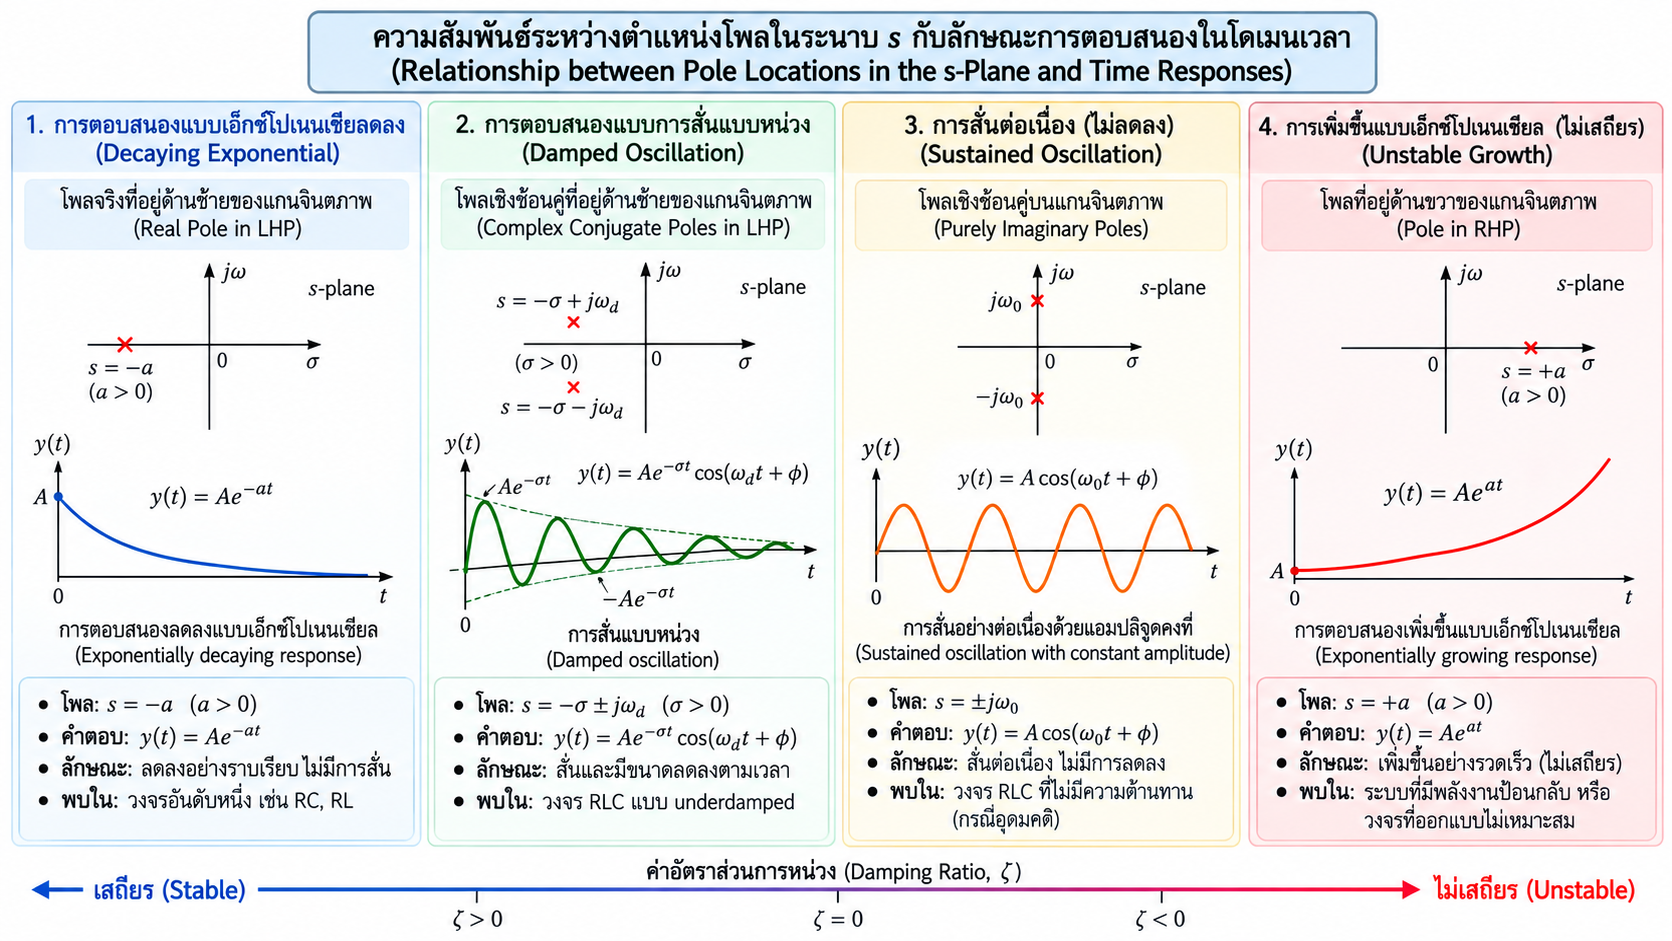
\includegraphics[width=0.8\textwidth]{images/chapter7/figure-08.png}
    \caption{ความสัมพันธ์ระหว่างตำแหน่งโพลกับรูปการตอบสนองเวลา}
\end{figure}

\par\noindent\rule{\textwidth}{0.4pt}\par

\paragraph{7.10.6 แนวทางตรวจสอบคำตอบด้วยทฤษฎีค่าเริ่มต้นและค่าปลายทาง}

แม้ว่าการหาลาปลาซผกผันจะให้คำตอบ $v(t)$ หรือ $i(t)$ แล้ว การตรวจสอบด้วย \textbf{Initial Value Theorem} และ \textbf{Final Value Theorem} ช่วยจับข้อผิดพลาดจากการแยกเศษส่วนหรือเครื่องหมายได้

\paragraph{7.11.1 Initial Value Theorem}

ภายใต้เงื่อนไขที่เหมาะสม

\[
\boxed{f(0^+)=\lim_{s\to\infty}sF(s)}
\]

ตัวอย่าง RC step

\[
V_C(s)=\frac{V_0}{s(RCs+1)}
\]

ดังนั้น

\[
\begin{aligned}
    \lim_{s\to\infty}sV_C(s) \\
    &=\lim_{s\to\infty}\frac{V_0}{RCs+1}=0
\end{aligned}
\]

สอดคล้องกับ $v_C(0^+)=0$

\paragraph{7.11.2 Final Value Theorem}

หากโพลของ $sF(s)$ ทั้งหมดอยู่ในครึ่งระนาบซ้ายอย่างเหมาะสม

\[
\boxed{f(\infty)=\lim_{s\to0}sF(s)}
\]

สำหรับ RC step

\[
\lim_{s\to0}sV_C(s)=\lim_{s\to0}\frac{V_0}{RCs+1}=V_0
\]

\textbf{ข้อจำกัด:} ห้ามใช้ Final Value Theorem แบบอัตโนมัติกับระบบที่ไม่เสถียรหรือมีการสั่นไม่ลดลง เพราะลิมิตเวลาอาจไม่มีอยู่จริง

\subsubsection{7.11 ตัวอย่างโจทย์และการคำนวณแบบเป็นขั้นตอน}

เพื่อให้การเรียนรู้เชื่อมจากหลักการไปสู่การแก้ปัญหา เนื้อหาในหัวข้อ 7.5–7.10 ได้สอดแทรก \textbf{ตัวอย่างเพิ่มเติมเพื่อการเรียนรู้จำนวน 7 ตัวอย่าง} เรียงจากวงจรอันดับหนึ่งไปสู่วงจรอันดับสองและการวิเคราะห์ระบบ ได้แก่

\begin{enumerate}
    \item การชาร์จตัวเก็บประจุในวงจร RC และการตีความ $\tau$
    \item วงจร RC ที่มีแรงดันเริ่มต้นไม่เป็นศูนย์
    \item การสร้างกระแสในวงจร RL
    \item การจำแนก underdamped / critically damped / overdamped ของ RLC
    \item การหาการตอบสนองขั้นบันไดของ RLC แบบ underdamped
    \item การหา transfer function, pole และ time constant ของ RC
    \item การหา poles, zero และประเมินเสถียรภาพจาก transfer function
\end{enumerate}

ทุกตัวอย่างใช้ลำดับคิดตาม Module B ได้แก่ วิเคราะห์ระบบ กำหนดตัวแปร เลือกหลักการ สร้างสมการ จัดรูป แปลงโดเมน/แทนค่า คำนวณ ตรวจสอบหน่วยและค่าขอบเขต และแปลความหมายทางกายภาพของคำตอบ

\subsubsection{7.12 กิจกรรมการเรียนรู้และแบบฝึกหัดท้ายบท}

กิจกรรมและแบบฝึกหัดของบทนี้จัดแยกในหัวข้อ \textbf{11. กิจกรรมการเรียนรู้ในชั้นเรียน}, \textbf{12. คำถามทบทวน} และ \textbf{13. แบบฝึกหัดท้ายบท} เพื่อให้ใช้งานได้สะดวกในการสอนและสามารถตัดส่วนเฉลยออกเป็นเอกสารสำหรับนักศึกษาได้ แบบฝึกหัดแบ่งเป็นระดับพื้นฐาน 5 ข้อ ระดับวิเคราะห์ 5 ข้อ และระดับประยุกต์ใช้ 3 ข้อ ตามแนวทางของ Module E พร้อมเฉลยและการตีความคำตอบสำหรับผู้สอน

\par\noindent\rule{\textwidth}{0.4pt}\par

\subsection{8. ความเข้าใจผิดที่พบบ่อย}

\begin{table}[htbp]
    \centering
    \begin{tabularx}{\textwidth}{L{0.41\textwidth} Y}
        \hline
        \textbf{ความเข้าใจผิด} & \textbf{แนวคิดที่ถูกต้อง} \\
        \hline
        1. แปลง capacitor เป็น $1/(sC)$ ได้เสมอ & ใช้เป็น impedance ตรง ๆ เมื่อ initial condition เป็นศูนย์ หรือเมื่อผล initial condition ถูกแทนอย่างถูกต้องแล้ว \\
        2. แปลง inductor เป็น $sL$ ได้เสมอ & ต้องรวมเทอม $Li_L(0^-)$ เมื่อกระแสเริ่มต้นไม่เป็นศูนย์ \\
        3. $v_C$ และ $i_C$ ต่อเนื่องทั้งคู่ & โดยทั่วไป $v_C$ ต่อเนื่อง แต่ $i_C$ อาจเปลี่ยนฉับพลันได้ \\
        4. $v_L$ และ $i_L$ ต่อเนื่องทั้งคู่ & โดยทั่วไป $i_L$ ต่อเนื่อง แต่ $v_L$ อาจเปลี่ยนฉับพลันได้ \\
        5. Transfer function คือ $Y(s)/X(s)$ ในทุกกรณี & นิยาม transfer function ต้องกำหนด initial conditions เป็นศูนย์ \\
        6. โพลคือซีโรของตัวเศษ & โพลเป็นรากตัวส่วน ส่วนซีโรเป็นรากตัวเศษ \\
        7. ถ้าไม่มี oscillation แปลว่าระบบไม่มี transient & ระบบอันดับหนึ่งและ overdamped มี transient แบบเอ็กซ์โพเนนเชียลได้โดยไม่สั่น \\
        8. $s=j\omega$ เสมอ & โดยทั่วไป $s=\sigma+j\omega$; $s=j\omega$ เป็นกรณีพิเศษสำหรับ frequency response \\
        9. RLC ทุกตัวมี $R_{crit}=2\sqrt{L/C}$ & สูตรนี้ตรงกับ series RLC ในรูปแบบที่กำหนด ไม่ใช่ทุก topology \\
        10. โพลอยู่ซ้ายยิ่งใกล้แกนจินตภาพยิ่งเร็ว & ตรงกันข้าม โพลที่ใกล้แกนจินตภาพมักลดช้ากว่า \\
        11. Final Value Theorem ใช้ได้กับทุก $F(s)$ & ต้องตรวจสอบเงื่อนไขเสถียรภาพของ $sF(s)$ ก่อน \\
        12. การแยก natural/forced เหมือนกับ transient/steady-state ทุกกรณี & เป็นคนละมุมมอง แม้บางโจทย์ RC/RL step จะดูเหมือนตรงกัน \\
        \hline
    \end{tabularx}
\end{table}

\par\noindent\rule{\textwidth}{0.4pt}\par

\subsection{9. การประยุกต์ใช้ในงานจริง}

\subsubsection{9.1 วงจรตั้งเวลาและดีเลย์ด้วย RC}

วงจร RC ใช้สร้างการหน่วงเวลาสำหรับการรีเซตไมโครคอนโทรลเลอร์ การกรองสัญญาณ และการทำ soft-start แบบง่าย ค่าคงตัวเวลา $RC$ ช่วยประมาณเวลาที่แรงดันถึง threshold ที่กำหนดได้ การวิเคราะห์ด้วย Laplace ช่วยให้สามารถต่อยอดไปยังวงจรที่มีหลายพจน์หรือแหล่งกระตุ้นที่ไม่ใช่ DC คงที่

\subsubsection{9.2 กระแสขณะสวิตช์ของขดลวดและรีเลย์}

ขดลวดรีเลย์ โซลินอยด์ และมอเตอร์มีอินดักแตนซ์ เมื่อป้อนแรงดัน กระแสไม่เพิ่มทันที แต่เพิ่มตาม $L/R$ time constant ส่วนเมื่อเปิดวงจร พลังงานในสนามแม่เหล็กต้องถูกระบาย จึงอาจเกิดแรงดันสูงที่ขั้วขดลวด วงจรป้องกันเช่น diode หรือ snubber เปลี่ยนเส้นทางการสลายพลังงานและมีผลต่อ transient

\subsubsection{9.3 การออกแบบฟิลเตอร์อันดับหนึ่ง}

RC low-pass และ high-pass มี transfer function ที่สามารถอ่าน pole/zero ได้โดยตรง เช่น

\[
H_{LP}(s)=\frac{1}{RCs+1}
\]

จึงเห็นทั้ง time constant และความถี่มุม

\[
\omega_c=\frac{1}{RC}
\]

ซึ่งเชื่อมการตอบสนองเวลาและการตอบสนองความถี่ไว้ในพารามิเตอร์เดียวกัน

\subsubsection{9.4 การสั่นและการหน่วงในวงจร RLC}

วงจรที่มี L และ C อาจเกิด ringing หลังการสวิตช์ เช่น ในสายสัญญาณ เครือข่ายกรอง หรือวงจรพลังงาน ค่าความต้านทานและการสูญเสียเป็นตัวกำหนดการหน่วง หาก damping ต่ำเกินไปอาจเกิด overshoot สูง ส่วน damping มากเกินไปอาจทำให้ response ช้า

\subsubsection{9.5 แบบจำลองสำหรับระบบควบคุม}

Transfer function ที่ได้จากวงจรเป็นสะพานไปสู่รายวิชาระบบควบคุม ตัวอย่างเซนเซอร์ที่มี RC low-pass สามารถแทนเป็น

\[
G(s)=\frac{1}{\tau s+1}
\]

ทำให้สามารถวิเคราะห์ว่า time constant ของวงจรเซนเซอร์ส่งผลต่อความเร็วของระบบรวมอย่างไร

\subsubsection{9.6 การวิเคราะห์การสตาร์ตของแหล่งจ่ายและวงจรอิเล็กทรอนิกส์}

แม้ว่าวงจรจริงอาจมีอุปกรณ์ไม่เชิงเส้น แต่ในช่วงที่สามารถประมาณเป็นวงจรเชิงเส้นได้ การใช้ Laplace model ช่วยประเมิน inrush, charging transient, overshoot และ settling behavior ของส่วน RLC ได้ ก่อนพิจารณาแบบจำลองละเอียดขึ้น

\par\noindent\rule{\textwidth}{0.4pt}\par

\subsection{10. สรุปท้ายบท}

บทนี้แสดงให้เห็นว่าการแปลงลาปลาซเป็นวิธีรวม \textbf{คณิตศาสตร์ของสมการเชิงอนุพันธ์} เข้ากับ \textbf{พฤติกรรมทางกายภาพของวงจรไฟฟ้า} อย่างเป็นระบบ ประเด็นสำคัญมีดังนี้

\begin{enumerate}
    \item วงจร RC และ RL เป็นระบบอันดับหนึ่งในกรณีพื้นฐาน โดยมีค่าคงตัวเวลา
\end{enumerate}

\[
\tau_{RC}=RC,\qquad \tau_{RL}=\frac{L}{R}
\]

\begin{enumerate}
    \item วงจร RLC อนุกรมมีสมการอันดับสอง
\end{enumerate}

\[
LC\frac{d^2v_C}{dt^2}+RC\frac{dv_C}{dt}+v_C=v_s(t)
\]

และพารามิเตอร์สำคัญคือ

\[
\begin{aligned}
    \omega_n&=\frac{1}{\sqrt{LC}},\qquad \\
    \alpha&=\frac{R}{2L},\qquad \\
    \zeta&=\frac{R}{2}\sqrt{\frac{C}{L}}
\end{aligned}
\]

\begin{enumerate}
    \item การแปลงอนุพันธ์ต้องรวม initial condition เช่น
\end{enumerate}

\[
\mathcal{L}\{f'(t)\}=sF(s)-f(0^-)
\]

\begin{enumerate}
    \item ภายใต้ zero initial conditions
\end{enumerate}

\[
Z_R=R,\qquad Z_L=sL,\qquad Z_C=\frac{1}{sC}
\]

แต่เมื่อ initial conditions ไม่เป็นศูนย์ ต้องรวมแหล่งสมมูลหรือเทอมที่สอดคล้องในสมการ

\begin{enumerate}
    \item Transfer function นิยามเป็น
\end{enumerate}

\[
G(s)=\frac{Y(s)}{X(s)}
\]

ภายใต้ \textbf{initial conditions เป็นศูนย์}

\begin{enumerate}
    \item โพลเป็นรากของตัวส่วนและสัมพันธ์โดยตรงกับ natural modes ของระบบ ส่วนซีโรเป็นรากของตัวเศษและมีผลต่อรูปร่างการตอบสนอง
\end{enumerate}

\begin{enumerate}
    \item สำหรับระบบต่อเนื่องเชิงเส้นมาตรฐาน โพลทั้งหมดในครึ่งระนาบซ้ายสัมพันธ์กับการตอบสนองธรรมชาติที่ลดลง ส่วนโพลในครึ่งระนาบขวาทำให้เกิดองค์ประกอบที่เติบโต
\end{enumerate}

\begin{enumerate}
    \item การตรวจสอบคำตอบควรทำทั้งในเชิงคณิตศาสตร์และกายภาพ ได้แก่ ค่า $0^+$, ค่า $\infty$, หน่วย, ขั้วแรงดัน, ทิศทางกระแส และพฤติกรรมของ L/C ใน steady-state DC
\end{enumerate}

ความเข้าใจในบทนี้เป็นฐานสำคัญสำหรับการวิเคราะห์ระบบเชิงเส้น ฟังก์ชันถ่ายโอน ระบบควบคุม ฟิลเตอร์ และการใช้โปรแกรมคำนวณในบทถัดไป

\par\noindent\rule{\textwidth}{0.4pt}\par

\subsection{11. กิจกรรมการเรียนรู้ในชั้นเรียน}

กิจกรรมต่อไปนี้ออกแบบให้ใช้ได้ภายในชั่วโมงบรรยายโดยไม่ต้องใช้อุปกรณ์ปฏิบัติการเฉพาะ และสัมพันธ์กับผลลัพธ์การเรียนรู้ของบท

\subsubsection{กิจกรรมที่ 1: จากวงจรจริงสู่สมการและโดเมน \texorpdfstring{$s$}{s}}

ให้นักศึกษาทำงานเป็นคู่ รับแผนภาพวงจร RC หรือ RL ที่มีสวิตช์หนึ่งวงจร แล้วดำเนินการ 4 ขั้น ได้แก่ (1) ระบุ $0^-$ และ $0^+$ (2) เขียนสมการเวลา (3) แปลงเป็นสมการใน $s$ (4) อธิบายความหมายของโพล ใช้เวลาประมาณ 15 นาที จากนั้นเปรียบเทียบคำตอบระหว่างคู่

\textbf{CLO ที่เกี่ยวข้อง:} CLO1, CLO2, CLO5\\
\textbf{หลักฐาน:} สมการเวลา สมการ $s$-domain และคำอธิบาย pole 1–2 ประโยค

\subsubsection{กิจกรรมที่ 2: วิเคราะห์ข้อผิดพลาดเรื่อง initial conditions}

ผู้สอนแสดงคำตอบที่จงใจผิด เช่น แทน inductor ด้วย $sL$ ทั้งที่ $i_L(0^-)\neq0$ หรือกำหนด $v_C(0^+)=0$ ทั้งที่ capacitor มีประจุอยู่ ให้นักศึกษาระบุว่า “ผิดตรงไหน–ควรแก้อย่างไร–คำตอบจะเปลี่ยนทิศทางใด” ใช้เวลาประมาณ 10 นาที

\textbf{CLO ที่เกี่ยวข้อง:} CLO2, CLO3\\
\textbf{หลักฐาน:} คำอธิบายข้อผิดพลาดและสมการที่แก้ไข

\subsubsection{กิจกรรมที่ 3: อ่านกราฟแล้วทายตำแหน่งโพล}

แสดงกราฟ 4 แบบ ได้แก่ exponential decay เร็ว, exponential decay ช้า, damped oscillation และ growing response ให้นักศึกษาจับคู่กับแผนภาพ pole location ในระนาบ $s$ พร้อมให้เหตุผลเรื่องส่วนจริงและส่วนจินตภาพ ใช้เวลาประมาณ 15 นาที

\textbf{CLO ที่เกี่ยวข้อง:} CLO4, CLO6\\
\textbf{หลักฐาน:} การจับคู่กราฟ–โพลและเหตุผลเชิงกายภาพ

\par\noindent\rule{\textwidth}{0.4pt}\par

\subsection{12. คำถามทบทวน}

\begin{enumerate}
    \item เพราะเหตุใดการแปลงลาปลาซจึงเหมาะกับการวิเคราะห์วงจรที่มีการสวิตช์และมีสภาวะเริ่มต้นไม่เป็นศูนย์
    \item อธิบายความแตกต่างระหว่าง $v_C(0^-)$, $v_C(0^+)$ และ $v_C(\infty)$
    \item เหตุใดแรงดันตัวเก็บประจุและกระแสตัวเหนี่ยวนำจึงเป็นตัวแปรที่ต้องให้ความสำคัญเมื่อเกิดการสวิตช์
    \item ภายใต้เงื่อนไขใดจึงสามารถใช้ $Z_L=sL$ และ $Z_C=1/(sC)$ ได้โดยตรง
    \item เปรียบเทียบความหมายของ time constant ในวงจร RC และ RL
    \item อธิบายความแตกต่างระหว่าง natural response, forced response, transient response และ steady-state response
    \item เหตุใด transfer function จึงต้องนิยามภายใต้ initial conditions เป็นศูนย์
    \item ตำแหน่งของโพลจริงที่ $s=-2$ และ $s=-20$ แตกต่างกันอย่างไรในแง่ความเร็วของ transient
    \item เพราะเหตุใด RLC underdamped จึงเกิดการสั่น ขณะที่ critically damped และ overdamped ไม่สั่น
    \item Final Value Theorem มีประโยชน์อย่างไร และเพราะเหตุใดต้องตรวจสอบเสถียรภาพก่อนใช้งาน
\end{enumerate}

\par\noindent\rule{\textwidth}{0.4pt}\par

\subsection{13. แบบฝึกหัดท้ายบท}

\subsubsection{13.1 ระดับพื้นฐาน}

\textbf{ข้อ 1}\\
เขียนความสัมพันธ์ในโดเมน $s$ ของตัวต้านทาน $R$, ตัวเหนี่ยวนำ $L$ และตัวเก็บประจุ $C$ โดยระบุทั้งกรณีสภาวะเริ่มต้นเป็นศูนย์และสมการที่มี initial condition สำหรับ L และ C

\textbf{ข้อ 2}\\
วงจร RC มี $R=5\,\text{k}\Omega$ และ $C=20\,\mu\text{F}$ จงหา (ก) ค่าคงตัวเวลา (ข) โพลของวงจร RC low-pass และ (ค) เวลาประมาณ $5\tau$

\textbf{ข้อ 3}\\
วงจร RL อนุกรมมี $R=25\,\Omega$, $L=0.5\,\text{H}$ รับแหล่ง $50u(t)$ V และ $i_L(0^-)=0$ จงหา $\tau$, กระแสปลายทาง และสมการ $i(t)$

\textbf{ข้อ 4}\\
วงจร RLC อนุกรมมี $L=0.2\,\text{H}$, $C=500\,\mu\text{F}$ และ $R=20\,\Omega$ จงหา $\omega_n$, $\alpha$, $\zeta$ และจำแนกชนิดการหน่วง

\textbf{ข้อ 5}\\
วงจร RC low-pass มี $R=10\,\text{k}\Omega$ และ $C=1\,\mu\text{F}$ จงหา transfer function ในรูป $K/(s+a)$ พร้อมระบุ pole และ DC gain

\subsubsection{13.2 ระดับวิเคราะห์}

\textbf{ข้อ 6}\\
ตัวเก็บประจุ $C=100\,\mu\text{F}$ มีแรงดันเริ่มต้น 3 V และที่ $t=0$ ถูกต่อผ่าน $R=2\,\text{k}\Omega$ เข้ากับแหล่ง DC 9 V จงหา $v_C(t)$ และ $i(0^+)$ พร้อมตรวจสอบค่า $v_C(0^+)$ และ $v_C(\infty)$

\textbf{ข้อ 7}\\
ตัวเหนี่ยวนำ $L=0.5\,\text{H}$ มีกระแสเริ่มต้น $3\,\text{A}$ และหลัง $t=0$ ถูกปล่อยให้คายพลังงานผ่านตัวต้านทาน $R=10\,\Omega$ โดยไม่มีแหล่งจ่าย จงหา $i_L(t)$, $v_R(t)$ และเวลาที่กระแสลดเหลือ $10\%$ ของค่าเริ่มต้น

\textbf{ข้อ 8}\\
วงจร RLC อนุกรมมี $L=0.1\,\text{H}$ และ $C=100\,\mu\text{F}$ จงหา $R_{\text{crit}}$ และจำแนกการตอบสนองสำหรับ $R=10\,\Omega$, $R=R_{\text{crit}}$ และ $R=100\,\Omega$

\textbf{ข้อ 9}\\
สำหรับวงจร RLC อนุกรมที่รับ $V_s(s)$ และวัดเอาต์พุต $V_R(s)$ คร่อมตัวต้านทาน จงสร้าง transfer function $H_R(s)=V_R(s)/V_s(s)$ ภายใต้ zero initial conditions และระบุ finite zero กับ poles ในรูปพหุนาม

\textbf{ข้อ 10}\\
กำหนด transfer function

\[
G(s)=\frac{20(s+5)}{(s+1)(s+4)(s+10)}
\]

จงหา poles, zero, DC gain และระบุ pole ที่คาดว่าจะ dominant ที่สุด พร้อมอธิบายผลต่อ transient

\subsubsection{13.3 ระดับประยุกต์ใช้}

\textbf{ข้อ 11}\\
ต้องการออกแบบวงจร RC ให้แรงดัน capacitor จาก 0 V ถึง $90\%$ ของแรงดันขั้นบันไดภายใน 0.50 s หากเลือก $C=100\,\mu\text{F}$ จงคำนวณค่า $R$ ที่ต้องการโดยประมาณ และระบุ pole ของวงจร

\textbf{ข้อ 12}\\
ขดลวดรีเลย์ประมาณเป็นวงจร $R$–$L$ อนุกรม มี $R=40\,\Omega$ และ $L=0.20\,\text{H}$ ต่อกับแหล่ง 12 V ที่ $t=0$ จงหา (ก) $i(t)$ (ข) เวลาที่กระแสถึง $95\%$ ของค่าปลายทาง และ (ค) พลังงานแม่เหล็กที่เก็บใน L เมื่อเข้าสู่ steady state

\textbf{ข้อ 13}\\
วงจร RLC อนุกรมใช้เป็นเครือข่ายอันดับสอง มี $L=10\,\text{mH}$ และ $C=10\,\mu\text{F}$ ต้องการอัตราส่วนการหน่วง $\zeta=0.70$ จงหา $R$, $\omega_n$, ตำแหน่ง poles โดยประมาณ และอธิบายว่าการตอบสนองเป็น underdamped หรือไม่

\par\noindent\rule{\textwidth}{0.4pt}\par

\subsection{13.4 เฉลยและแนวคำตอบสำหรับผู้สอน}

\begin{quote}
ส่วนนี้แยกออกจากโจทย์เพื่อให้สามารถตัดออกได้เมื่อต้องการจัดทำเอกสารสำหรับนักศึกษา
\end{quote}

\subsubsection{เฉลยข้อ 1}

\textbf{แนวคิด:} ใช้ความสัมพันธ์แรงดัน–กระแสและสมบัติ Laplace ของอนุพันธ์

ตัวต้านทาน

\[
V_R(s)=RI_R(s),\qquad Z_R=R
\]

ตัวเหนี่ยวนำ

\[
V_L(s)=sLI_L(s)-Li_L(0^-)
\]

เมื่อ $i_L(0^-)=0$

\[
Z_L=sL
\]

ตัวเก็บประจุ

\[
I_C(s)=sCV_C(s)-Cv_C(0^-)
\]

หรือ

\[
V_C(s)=\frac{1}{sC}I_C(s)+\frac{v_C(0^-)}{s}
\]

เมื่อ $v_C(0^-)=0$

\[
Z_C=\frac{1}{sC}
\]

\textbf{การแปลความหมาย:} initial conditions ของ L และ C ต้องไม่ถูกละทิ้งหากไม่เป็นศูนย์

\subsubsection{เฉลยข้อ 2}

ให้

\[
R=5000\,\Omega,\qquad C=20\times10^{-6}\,\text{F}
\]

ค่าคงตัวเวลา

\[
\tau=RC=(5000)(20\times10^{-6})=0.10\,\text{s}
\]

โพลของ RC low-pass

\[
p=-\frac{1}{RC}=-10\,\text{s}^{-1}
\]

และ

\[
5\tau=0.50\,\text{s}
\]

ดังนั้น

\[
\boxed{\tau=0.10\,\text{s},\quad p=-10\,\text{s}^{-1},\quad5\tau=0.50\,\text{s}}
\]

\textbf{ตรวจสอบ:} โพลมีส่วนจริงลบ จึงได้ exponential decay ที่เสถียร

\subsubsection{เฉลยข้อ 3}

\[
\tau=\frac{L}{R}=\frac{0.5}{25}=0.020\,\text{s}
\]

กระแสปลายทาง

\[
I_f=\frac{50}{25}=2\,\text{A}
\]

เนื่องจาก initial current เป็นศูนย์

\[
i(t)=I_f(1-e^{-t/\tau})
\]

ดังนั้น

\[
\boxed{i(t)=2(1-e^{-50t})\ \text{A}}
\]

\textbf{ตรวจสอบ:} $i(0)=0$ และ $i(\infty)=2$ A

\subsubsection{เฉลยข้อ 4}

กำหนด

\[
L=0.2\,\text{H},\quad C=500\times10^{-6}\,\text{F},\quad R=20\,\Omega
\]

ความถี่ธรรมชาติ

\[
\begin{aligned}
    \omega_n&=\frac{1}{\sqrt{LC}} \\
    &=\frac{1}{\sqrt{(0.2)(500\times10^{-6})}}
\end{aligned}
\]

เนื่องจาก $LC=10^{-4}$

\[
\boxed{\omega_n=100\,\text{rad/s}}
\]

อัตราการลดทอน

\[
\alpha=\frac{R}{2L}=\frac{20}{0.4}=50\,\text{s}^{-1}
\]

อัตราส่วนการหน่วง

\[
\zeta=\frac{\alpha}{\omega_n}=\frac{50}{100}=0.5
\]

ดังนั้น

\[
\boxed{\zeta=0.5<1\Rightarrow \text{underdamped}}
\]

\textbf{ความหมาย:} คาดว่าจะมีการสั่นแบบลดลงก่อนเข้าสู่ค่าปลายทาง

\subsubsection{เฉลยข้อ 5}

\[
RC=(10^4)(10^{-6})=0.01\,\text{s}
\]

\[
H(s)=\frac{1}{0.01s+1}
\]

คูณเศษและส่วนด้วย 100

\[
\boxed{H(s)=\frac{100}{s+100}}
\]

pole

\[
\boxed{p=-100\,\text{s}^{-1}}
\]

DC gain

\[
H(0)=\frac{100}{100}=1
\]

ดังนั้น DC gain เท่ากับ 1

\subsubsection{เฉลยข้อ 6}

\textbf{1. Initial condition}

\[
v_C(0^+)=3\,\text{V}
\]

\textbf{2. Final value}

\[
V_f=9\,\text{V}
\]

\textbf{3. Time constant}

\[
\tau=RC=(2000)(100\times10^{-6})=0.2\,\text{s}
\]

\textbf{4. Response}

\[
v_C(t)=V_f+[V_0-V_f]e^{-t/\tau}
\]

\[
\boxed{v_C(t)=9-6e^{-5t}\ \text{V}}
\]

\textbf{5. Initial current}

\[
i(0^+)=\frac{9-3}{2000}=3\times10^{-3}\,\text{A}
\]

\[
\boxed{i(0^+)=3\,\text{mA}}
\]

\textbf{6. ตรวจสอบ}

\[
v_C(0)=9-6=3\,\text{V}
\]

และ

\[
v_C(\infty)=9\,\text{V}
\]

ถูกต้อง

\subsubsection{เฉลยข้อ 7}

เป็น source-free RL

\[
\tau=\frac{L}{R}=\frac{0.5}{10}=0.05\,\text{s}
\]

กระแส

\[
\boxed{i_L(t)=3e^{-t/0.05}=3e^{-20t}\ \text{A}}
\]

แรงดันคร่อมตัวต้านทานตามทิศกระแส

\[
\boxed{v_R(t)=Ri=30e^{-20t}\ \text{V}}
\]

ต้องการให้

\[
i_L(t)=0.1I_0
\]

\[
e^{-t/\tau}=0.1
\]

\[
t=-\tau\ln0.1=(0.05)(2.3026)
\]

\[
\boxed{t\approx0.115\,\text{s}}
\]

\textbf{ข้อสังเกต:} ขั้วแรงดันของตัวเหนี่ยวนำจะต้องสมดุลกับแรงดันตัวต้านทานตาม KVL และขึ้นกับ passive sign convention ที่กำหนด

\subsubsection{เฉลยข้อ 8}

\[
R_{crit}=2\sqrt{\frac{L}{C}}
\]

แทนค่า

\[
\begin{aligned}
    R_{crit}&=2\sqrt{\frac{0.1}{100\times10^{-6}}} \\
    &=2\sqrt{1000}
\end{aligned}
\]

\[
\boxed{R_{crit}\approx63.25\,\Omega}
\]

ดังนั้น

\begin{itemize}
    \item $R=10\,\Omega<63.25\,\Omega$ $\to$ underdamped
    \item $R=63.25\,\Omega$ $\to$ critically damped
    \item $R=100\,\Omega>63.25\,\Omega$ $\to$ overdamped
\end{itemize}

\subsubsection{เฉลยข้อ 9}

อิมพีแดนซ์รวม

\[
Z_{tot}=R+sL+\frac{1}{sC}
\]

กระแส

\[
I(s)=\frac{V_s(s)}{Z_{tot}}
\]

แรงดันคร่อม R

\[
V_R(s)=RI(s)
\]

ดังนั้น

\[
H_R(s)=\frac{R}{R+sL+1/(sC)}
\]

คูณด้วย $sC$

\[
\boxed{H_R(s)=\frac{RCs}{LCs^2+RCs+1}}
\]

finite zero เกิดจากตัวเศษ

\[
RCs=0\Rightarrow \boxed{z=0}
\]

poles เป็นรากของ

\[
\boxed{LCs^2+RCs+1=0}
\]

\textbf{ความหมาย:} เอาต์พุตคร่อม R เป็นศูนย์ที่ DC เพราะเมื่อ $s\to0$ กระแส steady-state ผ่าน series capacitor เป็นศูนย์

\subsubsection{เฉลยข้อ 10}

\[
G(s)=\frac{20(s+5)}{(s+1)(s+4)(s+10)}
\]

zero

\[
\boxed{z=-5}
\]

poles

\[
\boxed{p_1=-1,\quad p_2=-4,\quad p_3=-10}
\]

DC gain

\[
G(0)=\frac{20(5)}{(1)(4)(10)}=\frac{100}{40}=2.5
\]

\[
\boxed{G(0)=2.5}
\]

pole ที่อยู่ใกล้แกนจินตภาพที่สุดคือ $-1$ จึงลดช้าที่สุดและคาดว่าจะ dominant ที่สุด

\textbf{การตีความ:} response ช่วงท้ายมีแนวโน้มถูกกำหนดโดยพจน์ใกล้ $e^{-t}$ มากกว่าพจน์ $e^{-4t}$ หรือ $e^{-10t}$

\subsubsection{เฉลยข้อ 11}

สำหรับ RC charging จาก 0

\[
\frac{v_C(t)}{V_s}=1-e^{-t/\tau}
\]

กำหนดให้ $v_C/V_s=0.90$ ที่ $t=0.50$ s

\[
0.90=1-e^{-0.50/\tau}
\]

\[
e^{-0.50/\tau}=0.10
\]

ลอการิทึม

\[
-\frac{0.50}{\tau}=\ln0.10=-2.3026
\]

ดังนั้น

\[
\tau=\frac{0.50}{2.3026}\approx0.2171\,\text{s}
\]

เมื่อ $C=100\,\mu\text{F}$

\[
R=\frac{\tau}{C}=\frac{0.2171}{100\times10^{-6}}
\]

\[
\boxed{R\approx2171\,\Omega\approx2.17\,\text{k}\Omega}
\]

pole

\[
p=-\frac{1}{\tau}\approx-4.605\,\text{s}^{-1}
\]

\[
\boxed{p\approx-4.61\,\text{s}^{-1}}
\]

\textbf{การแปลความหมาย:} ในงานจริงอาจเลือกค่ามาตรฐานใกล้เคียงแล้วคำนวณเวลาใหม่จากค่าจริงของ R และ C รวม tolerance

\subsubsection{เฉลยข้อ 12}

ให้

\[
R=40\,\Omega,\quad L=0.20\,\text{H},\quad V=12\,\text{V}
\]

ค่าคงตัวเวลา

\[
\tau=\frac{L}{R}=\frac{0.20}{40}=0.005\,\text{s}=5\,\text{ms}
\]

กระแสปลายทาง

\[
I_f=\frac{12}{40}=0.30\,\text{A}
\]

ดังนั้น

\[
\boxed{i(t)=0.30(1-e^{-200t})\ \text{A}}
\]

สำหรับ 95\%

\[
0.95=1-e^{-t/\tau}
\]

\[
e^{-t/\tau}=0.05
\]

\[
t=-\tau\ln0.05=(0.005)(2.9957)
\]

\[
\boxed{t_{95}\approx0.01498\,\text{s}\approx15\,\text{ms}}
\]

พลังงานใน L ที่ steady state

\[
W_L=\frac{1}{2}LI_f^2
\]

\[
=\frac{1}{2}(0.20)(0.30)^2
\]

\[
\boxed{W_L=0.009\,\text{J}=9\,\text{mJ}}
\]

\textbf{ความหมายเชิงวิศวกรรม:} พลังงานนี้ต้องมีเส้นทางระบายเมื่อเปิดวงจร มิฉะนั้นแรงดันที่ขดลวดอาจสูงขึ้นมากเพื่อพยายามรักษากระแส

\subsubsection{เฉลยข้อ 13}

กำหนด

\[
L=10\,\text{mH}=0.01\,\text{H}
\]

\[
C=10\,\mu\text{F}=10^{-5}\,\text{F}
\]

และ $\zeta=0.70$

สำหรับ series RLC

\[
\zeta=\frac{R}{2}\sqrt{\frac{C}{L}}
\]

แก้หา R

\[
R=2\zeta\sqrt{\frac{L}{C}}
\]

\[
R=2(0.70)\sqrt{\frac{0.01}{10^{-5}}}
\]

\[
R=1.4\sqrt{1000}
\]

\[
\boxed{R\approx44.27\,\Omega}
\]

ความถี่ธรรมชาติ

\[
\begin{aligned}
    \omega_n&=\frac{1}{\sqrt{LC}} \\
    &=\frac{1}{\sqrt{10^{-7}}}
\end{aligned}
\]

\[
\boxed{\omega_n\approx3162.3\,\text{rad/s}}
\]

ส่วนจริงของโพล

\[
-\zeta\omega_n\approx-(0.70)(3162.3)=-2213.6
\]

ความถี่ damped

\[
\omega_d=\omega_n\sqrt{1-\zeta^2}
\]

\[
=3162.3\sqrt{1-0.49}
\]

\[
\approx3162.3(0.7141)\approx2258\,\text{rad/s}
\]

ดังนั้น poles

\[
\boxed{p_{1,2}\approx-2214\pm j2258\ \text{s}^{-1}}
\]

เพราะ $\zeta=0.70<1$ ระบบจึง \textbf{underdamped} และมีการสั่นแบบลดลง แต่การหน่วงค่อนข้างมากกว่ากรณี $\zeta$ ต่ำ เช่น 0.2

\par\noindent\rule{\textwidth}{0.4pt}\par

\subsection{14. ข้อเสนอแนะสำหรับผู้สอน}

\subsubsection{14.1 ลำดับการสอนที่แนะนำสำหรับ 3 ชั่วโมง}

\begin{table}[htbp]
    \centering
    \small
    \setlength{\tabcolsep}{4pt}
    \begin{tabularx}{\textwidth}{L{0.16\textwidth} L{0.34\textwidth} Y}
        \hline
        \textbf{ช่วงเวลาโดยประมาณ} & \textbf{เนื้อหา/กิจกรรม} & \textbf{จุดเน้น} \\
        \hline
        0–20 นาที & ทบทวน Laplace derivative property และ initial conditions & ให้ผู้เรียนเขียน $\mathcal{L}\{f'\}$ และ $\mathcal{L}\{f''\}$ ได้โดยไม่สับสน $0^-$ \\
        20–50 นาที & 7.1–7.4 แบบจำลองวงจรและ $s$-domain impedance & เน้นว่า $sL$, $1/(sC)$ ใช้ตรง ๆ เมื่อ IC เป็นศูนย์ \\
        50–80 นาที & RC และตัวอย่างที่ 1–2 & เชื่อม $\tau$, pole, initial/final value และกราฟ \\
        80–105 นาที & RL และตัวอย่างที่ 3 & เปรียบเทียบกับ RC โดยใช้โครงสร้างอันดับหนึ่งเดียวกัน \\
        105–145 นาที & RLC และตัวอย่างที่ 4–5 & เน้น $\omega_n$, $\zeta$, pole locations และสามชนิด damping \\
        145–165 นาที & Transfer function, poles, zeros, stability & เชื่อมไปสู่วิชาระบบควบคุมและบทที่ 8 \\
        165–180 นาที & กิจกรรมอ่านกราฟ–ทายโพล + exit question & ประเมิน CLO4–CLO6 แบบ formative \\
        \hline
    \end{tabularx}
\end{table}

ผู้สอนสามารถลดจำนวนขั้นคำนวณในตัวอย่างที่ 5 หากเวลาไม่เพียงพอ แล้วมอบเป็นโจทย์หลังเรียน โดยควรรักษาเวลาอภิปรายเรื่อง \textbf{initial conditions และ pole interpretation} เพราะเป็นสองจุดที่ผู้เรียนมักผิดมากที่สุด

\subsubsection{14.2 จุดที่ควรเน้นระหว่างสอน}

\begin{enumerate}
    \item \textbf{เริ่มจากวงจร $t<0$ ก่อนเสมอ} ในโจทย์สวิตช์ ไม่ควรรีบวาด $s$-domain circuit ก่อนหา initial conditions
    \item ให้ผู้เรียนพูดออกเสียงว่า “แรงดัน C ต่อเนื่อง กระแส L ต่อเนื่อง” ก่อนเริ่มโจทย์ 2–3 ครั้ง เพื่อสร้าง mental model ที่ถูกต้อง
    \item เมื่อได้คำตอบ $v(t)$ หรือ $i(t)$ ให้ตรวจ $t=0^+$ และ $t\to\infty$ ทุกครั้ง ไม่ควรจบที่การแยกเศษส่วนย่อย
    \item สอน RC และ RL ด้วยรูปแบบเดียวกัน
\end{enumerate}

\[
\boxed{x(t)=x_f+[x(0^+)-x_f]e^{-t/\tau}}
\]

เพื่อให้ผู้เรียนเห็นโครงสร้างระบบอันดับหนึ่งร่วมกัน

\begin{enumerate}
    \item ก่อนสอน RLC ให้ย้ำว่าระบบอันดับสองมีพลังงานสองแหล่งและมีโพลสองตัว จึงเกิดพฤติกรรมที่วงจรอันดับหนึ่งไม่มี เช่น ringing และ damping regimes
    \item ในหัวข้อ transfer function ให้เขียนคำว่า \textbf{zero initial conditions} ไว้ข้างนิยามทุกครั้ง
    \item ในหัวข้อ stability ควรใช้ระนาบ $s$ คู่กับกราฟเวลาเสมอ ไม่ควรสอนเป็นกฎจำ “ซ้ายดี–ขวาไม่ดี” โดยไม่มีเหตุผลจาก $e^{st}$
\end{enumerate}

\subsubsection{14.3 เทคนิคประเมินระหว่างเรียน}

\textbf{คำถามเร็ว 1:} หาก $v_C(0^-)=5$ V แล้วสวิตช์เปลี่ยนที่ $t=0$ ค่า $v_C(0^+)$ เป็นเท่าใดในวงจรปกติที่ไม่มี impulse?\\
\textbf{คำตอบคาดหวัง:} 5 V

\textbf{คำถามเร็ว 2:} หาก $G(s)=10/(s+20)$ ค่า time constant โดยประมาณเท่าใด?\\
\textbf{คำตอบคาดหวัง:} $1/20=0.05$ s

\textbf{คำถามเร็ว 3:} โพล $-2\pm j10$ บอกอะไรเกี่ยวกับ response?\\
\textbf{คำตอบคาดหวัง:} มี damped oscillation ซองลดประมาณ $e^{-2t}$ และความถี่การสั่นประมาณ 10 rad/s

\textbf{คำถามเร็ว 4:} Transfer function สามารถรวมผล $v_C(0^-)=3$ V เป็นส่วนหนึ่งของนิยามได้หรือไม่?\\
\textbf{คำตอบคาดหวัง:} ไม่ได้ นิยาม transfer function ใช้ zero initial conditions; ผล initial state ต้องวิเคราะห์แยก

\subsubsection{14.4 เกณฑ์ประเมินโจทย์คำนวณแบบ OBE}

ตัวอย่าง rubric 10 คะแนนสำหรับโจทย์วิเคราะห์หนึ่งข้อ

\begin{table}[htbp]
    \centering
    \begin{tabularx}{\textwidth}{L{0.34\textwidth} r Y}
        \hline
        \textbf{เกณฑ์} & \textbf{คะแนน} & \textbf{หลักฐานที่คาดหวัง} \\
        \hline
        วิเคราะห์วงจรและกำหนด initial conditions & 2 & ระบุ $0^-$/$0^+$ ถูกต้องและกำหนดขั้ว/ทิศทางชัดเจน \\
        สร้างสมการหรือวงจร $s$-domain & 2 & ใช้ KVL/KCL และโมเดล RLC ถูกต้อง \\
        จัดรูปและแก้ $V(s)$ หรือ $I(s)$ & 2 & พีชคณิตถูกต้องและมีหน่วย/พารามิเตอร์เหมาะสม \\
        Inverse Laplace & 2 & แยกเศษส่วนและได้คำตอบเวลาอย่างถูกต้อง \\
        ตรวจสอบและตีความ & 2 & ตรวจ initial/final value, pole/time constant และอธิบายพฤติกรรมได้ \\
        \hline
    \end{tabularx}
\end{table}

Rubric นี้ให้ความสำคัญกับ \textbf{กระบวนการวิเคราะห์} ไม่ใช่เฉพาะคำตอบสุดท้าย จึงสอดคล้องกับ CLO ที่ใช้คำกริยา “สร้างแบบจำลอง วิเคราะห์ คำนวณ และประเมิน”

\subsubsection{14.5 การปรับระดับสำหรับผู้เรียนพื้นฐานต่างกัน}

\begin{itemize}
    \item \textbf{ผู้เรียนที่ยังไม่คล่อง Laplace:} ให้ตารางคู่ transform/inverse transform และเน้นโจทย์ RC/RL ก่อน RLC
    \item \textbf{ผู้เรียนระดับกลาง:} ให้โจทย์ initial condition ไม่เป็นศูนย์และโจทย์หา transfer function จากวงจร
    \item \textbf{ผู้เรียนที่พร้อมก้าวหน้า:} ให้โจทย์ pole–zero interpretation และการประมาณ dominant pole โดยไม่ต้องใช้ซอฟต์แวร์
    \item ควรหลีกเลี่ยงการเพิ่ม root locus, Bode design หรือ state-space แบบเต็มรูปแบบในบทนี้ เพราะเกินขอบเขตที่กำหนดและเป็นเนื้อหาของรายวิชาระบบควบคุมมากกว่า
\end{itemize}

\par\noindent\rule{\textwidth}{0.4pt}\par

\subsection{15. สื่อและแหล่งเรียนรู้เพิ่มเติม}

รายการต่อไปนี้เป็น \textbf{สื่อแนะนำ} สำหรับเสริมการสอน ไม่ใช่รายการอ้างอิงหลักของเนื้อหา ผู้สอนควรตรวจสอบหน้าเว็บและความพร้อมใช้งานก่อนนำไปใช้จริง

\begin{table}[htbp]
    \centering
    \scriptsize
    \setlength{\tabcolsep}{3pt}
    \begin{tabularx}{\textwidth}{L{0.24\textwidth} L{0.15\textwidth} L{0.22\textwidth} Y L{0.15\textwidth}}
        \hline
        \textbf{องค์กร/ผู้จัดทำ} & \textbf{หัวข้อที่ควรค้น} & \textbf{คำค้นแนะนำ} & \textbf{จุดประสงค์ในการรับชม/อ่าน} & \textbf{ช่วงเวลาที่เหมาะสม} \\
        \hline
        MIT OpenCourseWare – Circuits and Electronics / Introduction to Electronics, Signals and Measurement & RC/RL transient response & \texttt{MIT OCW transient analysis RC RL circuits} & ดูที่มาของ first-order differential equations, time constants และ transient graphs & ก่อนหรือหลังหัวข้อ 7.5–7.6 \\
        MIT OpenCourseWare – Differential Equations & RLC circuits and damping ratio & \texttt{MIT OCW RLC circuits damping ratio differential equations} & เชื่อมสมการอันดับสองกับ under/critical/over damping & ประกอบหัวข้อ 7.7 \\
        MIT OpenCourseWare – Electronic Feedback Systems & Laplace transforms and linear systems & \texttt{MIT OCW Laplace transform linear time invariant systems} & เชื่อม Laplace transform กับระบบ LTI และการตอบสนอง & หลังหัวข้อ 7.8 \\
        MathWorks Documentation & Transfer function models, poles and zeros & \texttt{MathWorks transfer function models poles zeros} & ตรวจนิยาม transfer function และศัพท์ pole/zero ในบริบท continuous-time systems & ประกอบหัวข้อ 7.9–7.10 \\
        Control Tutorials for MATLAB and Simulink, University of Michigan & System modeling and system analysis & \texttt{CTMS system modeling transfer function poles zeros stability} & ดูตัวอย่างการตีความ pole locations กับ system response & หลังหัวข้อ 7.10 หรือเตรียมเข้าสู่วิชาระบบควบคุม \\
        \hline
    \end{tabularx}
\end{table}

\subsubsection{15.1 แนวทางใช้สื่ออย่างมีเป้าหมาย}

ผู้สอนไม่ควรเปิดวิดีโอหรือสื่อออนไลน์ยาวทั้งช่วงเรียน แต่ควรกำหนด “คำถามนำ” เช่น

\begin{itemize}
    \item จากกราฟ RC ในสื่อ จุด $t=\tau$ มีความหมายอย่างไร?
    \item ใน RLC ถ้าเพิ่ม R เหตุใดการสั่นจึงลดลง?
    \item ใน transfer function ตัวส่วนสัมพันธ์กับสมการลักษณะเฉพาะอย่างไร?
    \item เมื่อ pole เคลื่อนเข้าใกล้แกนจินตภาพ transient ช้าลงหรือเร็วขึ้น?
\end{itemize}

จากนั้นให้ผู้เรียนสรุปเป็น 2–3 ประโยคหรือวาดภาพประกอบสั้น ๆ เพื่อให้การรับชมสื่อเกิดการเรียนรู้เชิงรุก

\par\noindent\rule{\textwidth}{0.4pt}\par

\subsection{16. เอกสารอ้างอิง}

ใช้รูปแบบ APA 7 และแยกตามประเภทแหล่งข้อมูล

\subsubsection{16.1 เอกสารหลักที่ผู้ใช้แนบ}

\begin{itemize}
    \item โครงสร้างเอกสารประกอบการสอน รายวิชา 5571102 คณิตศาสตร์วิศวกรรมไฟฟ้า. (2569). \textit{เอกสารโครงสร้างรายวิชาและสารบัญสำหรับจัดทำเอกสารประกอบการสอน} [เอกสารภายใน].
    \item \textit{Prompt กลางสำหรับออกแบบเอกสารประกอบการสอนระดับอุดมศึกษา}. (ม.ป.ป.). [เอกสารแนวทางการออกแบบ].
    \item \textit{Module A: ภาพประกอบและ Prompt สร้างภาพ}. (ม.ป.ป.). [เอกสารแนวทาง].
    \item \textit{Module B: สมการและตัวอย่างคำนวณ}. (ม.ป.ป.). [เอกสารแนวทาง].
    \item \textit{Module E: แบบฝึกหัดและเฉลย}. (ม.ป.ป.). [เอกสารแนวทาง].
    \item \textit{Module F: OBE และการประเมินผล}. (ม.ป.ป.). [เอกสารแนวทาง].
    \item \textit{Module H: สื่อ วิดีโอ และเอกสารอ้างอิง}. (ม.ป.ป.). [เอกสารแนวทาง].
\end{itemize}

\subsubsection{16.2 หนังสือและตำรา}

\begin{itemize}
    \item Alexander, C. K., \& Sadiku, M. N. O. (2021). \textit{Fundamentals of electric circuits} (7th ed.). McGraw Hill.
    \item Nilsson, J. W., \& Riedel, S. A. (2024). \textit{Electric circuits} (12th ed., Global ed.). Pearson.
\end{itemize}

\subsubsection{16.3 เอกสารวิชาการและเอกสารการสอนจากมหาวิทยาลัย}

\begin{itemize}
    \item Chaniotakis, M., \& Cory, D. (2006). \textit{Transient analysis of first order RC and RL circuits}. MIT OpenCourseWare, Massachusetts Institute of Technology, course 6.071J/22.071J Introduction to Electronics, Signals and Measurement.
    \item Chaniotakis, M., \& Cory, D. (2006). \textit{The RLC circuit: Transient response}. MIT OpenCourseWare, Massachusetts Institute of Technology, course 6.071J/22.071J Introduction to Electronics, Signals and Measurement.
    \item Massachusetts Institute of Technology OpenCourseWare. (2011). \textit{Applications: LRC circuits}. 18.03SC Differential Equations.
\end{itemize}

\subsubsection{16.4 เอกสารทางเทคนิคและแหล่งข้อมูลออนไลน์}

\begin{itemize}
    \item The MathWorks, Inc. (n.d.). \textit{What are transfer function models?} MATLAB \& Simulink documentation. สืบค้นเมื่อ 19 สิงหาคม 2026.
    \item Control Tutorials for MATLAB and Simulink, University of Michigan. (n.d.). \textit{Introduction: System modeling} และ \textit{Introduction: System analysis}. สืบค้นเมื่อ 19 สิงหาคม 2026.
\end{itemize}

\subsubsection{16.5 หมายเหตุด้านการอ้างอิง}

\begin{enumerate}
    \item รายการตำรา Alexander \& Sadiku และ Nilsson \& Riedel ได้ตรวจสอบข้อมูลรุ่นและสำนักพิมพ์จากหน้าสำนักพิมพ์ในช่วงจัดทำต้นฉบับ
    \item เอกสาร MIT OpenCourseWare ที่ใช้ประกอบการตรวจสอบหลักการ RC/RL/RLC แสดงสมการ differential equation, time constant และ damping behavior ที่สอดคล้องกับเนื้อหาในบทนี้
    \item เอกสาร MathWorks ใช้ประกอบการตรวจสอบนิยาม transfer-function model และความหมายของ roots ของ numerator/denominator ในฐานะ zeros/poles
    \item ก่อนเผยแพร่เอกสารฉบับพิมพ์ ผู้สอนควรตรวจรูปแบบบรรณานุกรม ชื่อรุ่น ISBN และสถานะหน้าเว็บอีกครั้งตามแนวปฏิบัติของสถาบัน
\end{enumerate}

\par\noindent\rule{\textwidth}{0.4pt}\par

\subsection{ภาคสรุปสมการสำคัญของบท}

\begin{table}[htbp]
    \centering
    \begin{tabular}{l l}
        \hline
        \textbf{หัวข้อ} & \textbf{สมการสำคัญ} \\
        \hline
        RC differential equation & $RC\,dv_C/dt+v_C=v_s$ \\
        RC time constant & $\tau=RC$ \\
        RC step response & $v_C(t)=V_f+[v_C(0^+)-V_f]e^{-t/\tau}$ \\
        RL differential equation & $L\,di/dt+Ri=v_s$ \\
        RL time constant & $\tau=L/R$ \\
        RL step response & $i_L(t)=I_f+[i_L(0^+)-I_f]e^{-t/\tau}$ \\
        Series RLC differential equation & $LC\,d^2v_C/dt^2+RC\,dv_C/dt+v_C=v_s$ \\
        Natural frequency & $\omega_n=1/\sqrt{LC}$ \\
        Damping rate & $\alpha=R/(2L)$ \\
        Damping ratio & $\zeta=(R/2)\sqrt{C/L}$ \\
        Critical resistance, series RLC & $R_{crit}=2\sqrt{L/C}$ \\
        Damped natural frequency & $\omega_d=\omega_n\sqrt{1-\zeta^2}$ \\
        Resistor $s$-domain & $Z_R=R$ \\
        Inductor with IC & $V_L=sLI_L-Li_L(0^-)$ \\
        Capacitor with IC & $I_C=sCV_C-Cv_C(0^-)$ \\
        Inductor zero-IC impedance & $Z_L=sL$ \\
        Capacitor zero-IC impedance & $Z_C=1/(sC)$ \\
        Transfer function & $G(s)=Y(s)/X(s)$ เมื่อ initial conditions เป็นศูนย์ \\
        Initial Value Theorem & $f(0^+)=\lim_{s\to\infty}sF(s)$ \\
        Final Value Theorem & $f(\infty)=\lim_{s\to0}sF(s)$ เมื่อเงื่อนไขเสถียรภาพเหมาะสม \\
        \hline
    \end{tabular}
\end{table}

\par\noindent\rule{\textwidth}{0.4pt}\par

\textbf{จบบทที่ 7 การประยุกต์การแปลงลาปลาซในการวิเคราะห์วงจรไฟฟ้า}
